% Options for packages loaded elsewhere
% Options for packages loaded elsewhere
\PassOptionsToPackage{unicode}{hyperref}
\PassOptionsToPackage{hyphens}{url}
\PassOptionsToPackage{dvipsnames,svgnames,x11names}{xcolor}
%
\documentclass[
  letterpaper,
  DIV=11,
  numbers=noendperiod]{scrartcl}
\usepackage{xcolor}
\usepackage{amsmath,amssymb}
\setcounter{secnumdepth}{-\maxdimen} % remove section numbering
\usepackage{iftex}
\ifPDFTeX
  \usepackage[T1]{fontenc}
  \usepackage[utf8]{inputenc}
  \usepackage{textcomp} % provide euro and other symbols
\else % if luatex or xetex
  \usepackage{unicode-math} % this also loads fontspec
  \defaultfontfeatures{Scale=MatchLowercase}
  \defaultfontfeatures[\rmfamily]{Ligatures=TeX,Scale=1}
\fi
\usepackage{lmodern}
\ifPDFTeX\else
  % xetex/luatex font selection
\fi
% Use upquote if available, for straight quotes in verbatim environments
\IfFileExists{upquote.sty}{\usepackage{upquote}}{}
\IfFileExists{microtype.sty}{% use microtype if available
  \usepackage[]{microtype}
  \UseMicrotypeSet[protrusion]{basicmath} % disable protrusion for tt fonts
}{}
\makeatletter
\@ifundefined{KOMAClassName}{% if non-KOMA class
  \IfFileExists{parskip.sty}{%
    \usepackage{parskip}
  }{% else
    \setlength{\parindent}{0pt}
    \setlength{\parskip}{6pt plus 2pt minus 1pt}}
}{% if KOMA class
  \KOMAoptions{parskip=half}}
\makeatother
% Make \paragraph and \subparagraph free-standing
\makeatletter
\ifx\paragraph\undefined\else
  \let\oldparagraph\paragraph
  \renewcommand{\paragraph}{
    \@ifstar
      \xxxParagraphStar
      \xxxParagraphNoStar
  }
  \newcommand{\xxxParagraphStar}[1]{\oldparagraph*{#1}\mbox{}}
  \newcommand{\xxxParagraphNoStar}[1]{\oldparagraph{#1}\mbox{}}
\fi
\ifx\subparagraph\undefined\else
  \let\oldsubparagraph\subparagraph
  \renewcommand{\subparagraph}{
    \@ifstar
      \xxxSubParagraphStar
      \xxxSubParagraphNoStar
  }
  \newcommand{\xxxSubParagraphStar}[1]{\oldsubparagraph*{#1}\mbox{}}
  \newcommand{\xxxSubParagraphNoStar}[1]{\oldsubparagraph{#1}\mbox{}}
\fi
\makeatother

\usepackage{color}
\usepackage{fancyvrb}
\newcommand{\VerbBar}{|}
\newcommand{\VERB}{\Verb[commandchars=\\\{\}]}
\DefineVerbatimEnvironment{Highlighting}{Verbatim}{commandchars=\\\{\}}
% Add ',fontsize=\small' for more characters per line
\usepackage{framed}
\definecolor{shadecolor}{RGB}{241,243,245}
\newenvironment{Shaded}{\begin{snugshade}}{\end{snugshade}}
\newcommand{\AlertTok}[1]{\textcolor[rgb]{0.68,0.00,0.00}{#1}}
\newcommand{\AnnotationTok}[1]{\textcolor[rgb]{0.37,0.37,0.37}{#1}}
\newcommand{\AttributeTok}[1]{\textcolor[rgb]{0.40,0.45,0.13}{#1}}
\newcommand{\BaseNTok}[1]{\textcolor[rgb]{0.68,0.00,0.00}{#1}}
\newcommand{\BuiltInTok}[1]{\textcolor[rgb]{0.00,0.23,0.31}{#1}}
\newcommand{\CharTok}[1]{\textcolor[rgb]{0.13,0.47,0.30}{#1}}
\newcommand{\CommentTok}[1]{\textcolor[rgb]{0.37,0.37,0.37}{#1}}
\newcommand{\CommentVarTok}[1]{\textcolor[rgb]{0.37,0.37,0.37}{\textit{#1}}}
\newcommand{\ConstantTok}[1]{\textcolor[rgb]{0.56,0.35,0.01}{#1}}
\newcommand{\ControlFlowTok}[1]{\textcolor[rgb]{0.00,0.23,0.31}{\textbf{#1}}}
\newcommand{\DataTypeTok}[1]{\textcolor[rgb]{0.68,0.00,0.00}{#1}}
\newcommand{\DecValTok}[1]{\textcolor[rgb]{0.68,0.00,0.00}{#1}}
\newcommand{\DocumentationTok}[1]{\textcolor[rgb]{0.37,0.37,0.37}{\textit{#1}}}
\newcommand{\ErrorTok}[1]{\textcolor[rgb]{0.68,0.00,0.00}{#1}}
\newcommand{\ExtensionTok}[1]{\textcolor[rgb]{0.00,0.23,0.31}{#1}}
\newcommand{\FloatTok}[1]{\textcolor[rgb]{0.68,0.00,0.00}{#1}}
\newcommand{\FunctionTok}[1]{\textcolor[rgb]{0.28,0.35,0.67}{#1}}
\newcommand{\ImportTok}[1]{\textcolor[rgb]{0.00,0.46,0.62}{#1}}
\newcommand{\InformationTok}[1]{\textcolor[rgb]{0.37,0.37,0.37}{#1}}
\newcommand{\KeywordTok}[1]{\textcolor[rgb]{0.00,0.23,0.31}{\textbf{#1}}}
\newcommand{\NormalTok}[1]{\textcolor[rgb]{0.00,0.23,0.31}{#1}}
\newcommand{\OperatorTok}[1]{\textcolor[rgb]{0.37,0.37,0.37}{#1}}
\newcommand{\OtherTok}[1]{\textcolor[rgb]{0.00,0.23,0.31}{#1}}
\newcommand{\PreprocessorTok}[1]{\textcolor[rgb]{0.68,0.00,0.00}{#1}}
\newcommand{\RegionMarkerTok}[1]{\textcolor[rgb]{0.00,0.23,0.31}{#1}}
\newcommand{\SpecialCharTok}[1]{\textcolor[rgb]{0.37,0.37,0.37}{#1}}
\newcommand{\SpecialStringTok}[1]{\textcolor[rgb]{0.13,0.47,0.30}{#1}}
\newcommand{\StringTok}[1]{\textcolor[rgb]{0.13,0.47,0.30}{#1}}
\newcommand{\VariableTok}[1]{\textcolor[rgb]{0.07,0.07,0.07}{#1}}
\newcommand{\VerbatimStringTok}[1]{\textcolor[rgb]{0.13,0.47,0.30}{#1}}
\newcommand{\WarningTok}[1]{\textcolor[rgb]{0.37,0.37,0.37}{\textit{#1}}}

\usepackage{longtable,booktabs,array}
\usepackage{calc} % for calculating minipage widths
% Correct order of tables after \paragraph or \subparagraph
\usepackage{etoolbox}
\makeatletter
\patchcmd\longtable{\par}{\if@noskipsec\mbox{}\fi\par}{}{}
\makeatother
% Allow footnotes in longtable head/foot
\IfFileExists{footnotehyper.sty}{\usepackage{footnotehyper}}{\usepackage{footnote}}
\makesavenoteenv{longtable}
\usepackage{graphicx}
\makeatletter
\newsavebox\pandoc@box
\newcommand*\pandocbounded[1]{% scales image to fit in text height/width
  \sbox\pandoc@box{#1}%
  \Gscale@div\@tempa{\textheight}{\dimexpr\ht\pandoc@box+\dp\pandoc@box\relax}%
  \Gscale@div\@tempb{\linewidth}{\wd\pandoc@box}%
  \ifdim\@tempb\p@<\@tempa\p@\let\@tempa\@tempb\fi% select the smaller of both
  \ifdim\@tempa\p@<\p@\scalebox{\@tempa}{\usebox\pandoc@box}%
  \else\usebox{\pandoc@box}%
  \fi%
}
% Set default figure placement to htbp
\def\fps@figure{htbp}
\makeatother





\setlength{\emergencystretch}{3em} % prevent overfull lines

\providecommand{\tightlist}{%
  \setlength{\itemsep}{0pt}\setlength{\parskip}{0pt}}



 


\KOMAoption{captions}{tableheading}
\makeatletter
\@ifpackageloaded{caption}{}{\usepackage{caption}}
\AtBeginDocument{%
\ifdefined\contentsname
  \renewcommand*\contentsname{Table of contents}
\else
  \newcommand\contentsname{Table of contents}
\fi
\ifdefined\listfigurename
  \renewcommand*\listfigurename{List of Figures}
\else
  \newcommand\listfigurename{List of Figures}
\fi
\ifdefined\listtablename
  \renewcommand*\listtablename{List of Tables}
\else
  \newcommand\listtablename{List of Tables}
\fi
\ifdefined\figurename
  \renewcommand*\figurename{Figure}
\else
  \newcommand\figurename{Figure}
\fi
\ifdefined\tablename
  \renewcommand*\tablename{Table}
\else
  \newcommand\tablename{Table}
\fi
}
\@ifpackageloaded{float}{}{\usepackage{float}}
\floatstyle{ruled}
\@ifundefined{c@chapter}{\newfloat{codelisting}{h}{lop}}{\newfloat{codelisting}{h}{lop}[chapter]}
\floatname{codelisting}{Listing}
\newcommand*\listoflistings{\listof{codelisting}{List of Listings}}
\makeatother
\makeatletter
\makeatother
\makeatletter
\@ifpackageloaded{caption}{}{\usepackage{caption}}
\@ifpackageloaded{subcaption}{}{\usepackage{subcaption}}
\makeatother
\usepackage{bookmark}
\IfFileExists{xurl.sty}{\usepackage{xurl}}{} % add URL line breaks if available
\urlstyle{same}
\hypersetup{
  pdftitle={Homework 7 Solutions},
  colorlinks=true,
  linkcolor={blue},
  filecolor={Maroon},
  citecolor={Blue},
  urlcolor={Blue},
  pdfcreator={LaTeX via pandoc}}


\title{Homework 7 Solutions}
\usepackage{etoolbox}
\makeatletter
\providecommand{\subtitle}[1]{% add subtitle to \maketitle
  \apptocmd{\@title}{\par {\large #1 \par}}{}{}
}
\makeatother
\subtitle{BSTA 551}
\author{}
\date{}
\begin{document}
\maketitle


\begin{center}\rule{0.5\linewidth}{0.5pt}\end{center}

\subsection{Problem 1: Two-Sample t-Tests for
Means}\label{problem-1-two-sample-t-tests-for-means}

\subsubsection{Part (a) --- Welch--Satterthwaite degrees of
freedom}\label{part-a-welchsatterthwaite-degrees-of-freedom}

Summary statistics:

\begin{Shaded}
\begin{Highlighting}[]
\NormalTok{n1 }\OtherTok{\textless{}{-}} \DecValTok{22}\NormalTok{; xbar1 }\OtherTok{\textless{}{-}} \FloatTok{412.8}\NormalTok{; s1 }\OtherTok{\textless{}{-}} \FloatTok{68.4}  \CommentTok{\# COPD}
\NormalTok{n2 }\OtherTok{\textless{}{-}} \DecValTok{25}\NormalTok{; xbar2 }\OtherTok{\textless{}{-}} \FloatTok{356.2}\NormalTok{; s2 }\OtherTok{\textless{}{-}} \FloatTok{41.7}  \CommentTok{\# Controls}

\CommentTok{\# Welch{-}Satterthwaite}
\NormalTok{v1 }\OtherTok{\textless{}{-}}\NormalTok{ s1}\SpecialCharTok{\^{}}\DecValTok{2} \SpecialCharTok{/}\NormalTok{ n1}
\NormalTok{v2 }\OtherTok{\textless{}{-}}\NormalTok{ s2}\SpecialCharTok{\^{}}\DecValTok{2} \SpecialCharTok{/}\NormalTok{ n2}

\NormalTok{nu\_hat }\OtherTok{\textless{}{-}}\NormalTok{ (v1 }\SpecialCharTok{+}\NormalTok{ v2)}\SpecialCharTok{\^{}}\DecValTok{2} \SpecialCharTok{/}\NormalTok{ (v1}\SpecialCharTok{\^{}}\DecValTok{2} \SpecialCharTok{/}\NormalTok{ (n1 }\SpecialCharTok{{-}} \DecValTok{1}\NormalTok{) }\SpecialCharTok{+}\NormalTok{ v2}\SpecialCharTok{\^{}}\DecValTok{2} \SpecialCharTok{/}\NormalTok{ (n2 }\SpecialCharTok{{-}} \DecValTok{1}\NormalTok{))}
\FunctionTok{cat}\NormalTok{(}\FunctionTok{sprintf}\NormalTok{(}\StringTok{"v1 = s1\^{}2/n1 = \%.4f}\SpecialCharTok{\textbackslash{}n}\StringTok{"}\NormalTok{, v1))}
\end{Highlighting}
\end{Shaded}

\begin{verbatim}
v1 = s1^2/n1 = 212.6618
\end{verbatim}

\begin{Shaded}
\begin{Highlighting}[]
\FunctionTok{cat}\NormalTok{(}\FunctionTok{sprintf}\NormalTok{(}\StringTok{"v2 = s2\^{}2/n2 = \%.4f}\SpecialCharTok{\textbackslash{}n}\StringTok{"}\NormalTok{, v2))}
\end{Highlighting}
\end{Shaded}

\begin{verbatim}
v2 = s2^2/n2 = 69.5556
\end{verbatim}

\begin{Shaded}
\begin{Highlighting}[]
\FunctionTok{cat}\NormalTok{(}\FunctionTok{sprintf}\NormalTok{(}\StringTok{"Numerator:   (v1 + v2)\^{}2 = \%.4f}\SpecialCharTok{\textbackslash{}n}\StringTok{"}\NormalTok{, (v1 }\SpecialCharTok{+}\NormalTok{ v2)}\SpecialCharTok{\^{}}\DecValTok{2}\NormalTok{))}
\end{Highlighting}
\end{Shaded}

\begin{verbatim}
Numerator:   (v1 + v2)^2 = 79646.6711
\end{verbatim}

\begin{Shaded}
\begin{Highlighting}[]
\FunctionTok{cat}\NormalTok{(}\FunctionTok{sprintf}\NormalTok{(}\StringTok{"Denominator: \%.4f}\SpecialCharTok{\textbackslash{}n}\StringTok{"}\NormalTok{, v1}\SpecialCharTok{\^{}}\DecValTok{2}\SpecialCharTok{/}\NormalTok{(n1}\DecValTok{{-}1}\NormalTok{) }\SpecialCharTok{+}\NormalTok{ v2}\SpecialCharTok{\^{}}\DecValTok{2}\SpecialCharTok{/}\NormalTok{(n2}\DecValTok{{-}1}\NormalTok{)))}
\end{Highlighting}
\end{Shaded}

\begin{verbatim}
Denominator: 2355.1563
\end{verbatim}

\begin{Shaded}
\begin{Highlighting}[]
\FunctionTok{cat}\NormalTok{(}\FunctionTok{sprintf}\NormalTok{(}\StringTok{"nu\_hat = \%.2f  {-}{-}\textgreater{}  round down to \%d}\SpecialCharTok{\textbackslash{}n}\StringTok{"}\NormalTok{, nu\_hat, }\FunctionTok{floor}\NormalTok{(nu\_hat)))}
\end{Highlighting}
\end{Shaded}

\begin{verbatim}
nu_hat = 33.82  -->  round down to 33
\end{verbatim}

\[\hat{\nu} = \frac{(s_1^2/n_1 + s_2^2/n_2)^2}{\dfrac{(s_1^2/n_1)^2}{n_1-1} + \dfrac{(s_2^2/n_2)^2}{n_2-1}}\]

The Welch--Satterthwaite approximation gives \(\hat{\nu} \approx 33.8\),
rounded down to \(33\) degrees of freedom.

\begin{center}\rule{0.5\linewidth}{0.5pt}\end{center}

\subsubsection{Part (b) --- Welch t-test
(one-sided)}\label{part-b-welch-t-test-one-sided}

\begin{Shaded}
\begin{Highlighting}[]
\NormalTok{SE\_diff }\OtherTok{\textless{}{-}} \FunctionTok{sqrt}\NormalTok{(s1}\SpecialCharTok{\^{}}\DecValTok{2}\SpecialCharTok{/}\NormalTok{n1 }\SpecialCharTok{+}\NormalTok{ s2}\SpecialCharTok{\^{}}\DecValTok{2}\SpecialCharTok{/}\NormalTok{n2)}
\NormalTok{t\_obs   }\OtherTok{\textless{}{-}}\NormalTok{ (xbar1 }\SpecialCharTok{{-}}\NormalTok{ xbar2) }\SpecialCharTok{/}\NormalTok{ SE\_diff}
\NormalTok{p\_one   }\OtherTok{\textless{}{-}} \FunctionTok{pt}\NormalTok{(t\_obs, }\AttributeTok{df =}\NormalTok{ nu\_hat, }\AttributeTok{lower.tail =} \ConstantTok{FALSE}\NormalTok{)}

\FunctionTok{cat}\NormalTok{(}\FunctionTok{sprintf}\NormalTok{(}\StringTok{"SE(xbar1 {-} xbar2) = \%.4f}\SpecialCharTok{\textbackslash{}n}\StringTok{"}\NormalTok{, SE\_diff))}
\end{Highlighting}
\end{Shaded}

\begin{verbatim}
SE(xbar1 - xbar2) = 16.7993
\end{verbatim}

\begin{Shaded}
\begin{Highlighting}[]
\FunctionTok{cat}\NormalTok{(}\FunctionTok{sprintf}\NormalTok{(}\StringTok{"t\_obs = \%.4f}\SpecialCharTok{\textbackslash{}n}\StringTok{"}\NormalTok{, t\_obs))}
\end{Highlighting}
\end{Shaded}

\begin{verbatim}
t_obs = 3.3692
\end{verbatim}

\begin{Shaded}
\begin{Highlighting}[]
\FunctionTok{cat}\NormalTok{(}\FunctionTok{sprintf}\NormalTok{(}\StringTok{"df    = \%.2f}\SpecialCharTok{\textbackslash{}n}\StringTok{"}\NormalTok{, nu\_hat))}
\end{Highlighting}
\end{Shaded}

\begin{verbatim}
df    = 33.82
\end{verbatim}

\begin{Shaded}
\begin{Highlighting}[]
\FunctionTok{cat}\NormalTok{(}\FunctionTok{sprintf}\NormalTok{(}\StringTok{"p{-}value (one{-}sided, upper) = \%.5f}\SpecialCharTok{\textbackslash{}n}\StringTok{"}\NormalTok{, p\_one))}
\end{Highlighting}
\end{Shaded}

\begin{verbatim}
p-value (one-sided, upper) = 0.00095
\end{verbatim}

\textbf{Test statistic:}
\(T_W = \dfrac{412.8 - 356.2}{\sqrt{68.4^2/22 + 41.7^2/25}} = 3.369\)

\textbf{Degrees of freedom:} \(\hat{\nu} \approx 33.8\)

\textbf{\(p\)-value:} \(\ensuremath{9.5\times 10^{-4}}\)

\textbf{Conclusion:} At \(\alpha = 0.05\) we reject \(H_0\)
(\(p < 0.05\)). There is statistically significant evidence that mean
plasma fibrinogen is higher in COPD patients than in healthy controls.

\begin{center}\rule{0.5\linewidth}{0.5pt}\end{center}

\subsubsection{Part (c) --- 95\% two-sided
CI}\label{part-c-95-two-sided-ci}

\begin{Shaded}
\begin{Highlighting}[]
\NormalTok{t\_crit }\OtherTok{\textless{}{-}} \FunctionTok{qt}\NormalTok{(}\FloatTok{0.975}\NormalTok{, }\AttributeTok{df =}\NormalTok{ nu\_hat)}
\NormalTok{ci\_lo  }\OtherTok{\textless{}{-}}\NormalTok{ (xbar1 }\SpecialCharTok{{-}}\NormalTok{ xbar2) }\SpecialCharTok{{-}}\NormalTok{ t\_crit }\SpecialCharTok{*}\NormalTok{ SE\_diff}
\NormalTok{ci\_hi  }\OtherTok{\textless{}{-}}\NormalTok{ (xbar1 }\SpecialCharTok{{-}}\NormalTok{ xbar2) }\SpecialCharTok{+}\NormalTok{ t\_crit }\SpecialCharTok{*}\NormalTok{ SE\_diff}

\FunctionTok{cat}\NormalTok{(}\FunctionTok{sprintf}\NormalTok{(}\StringTok{"t\_crit (df = \%.1f) = \%.4f}\SpecialCharTok{\textbackslash{}n}\StringTok{"}\NormalTok{, nu\_hat, t\_crit))}
\end{Highlighting}
\end{Shaded}

\begin{verbatim}
t_crit (df = 33.8) = 2.0326
\end{verbatim}

\begin{Shaded}
\begin{Highlighting}[]
\FunctionTok{cat}\NormalTok{(}\FunctionTok{sprintf}\NormalTok{(}\StringTok{"95\%\% CI: (\%.2f, \%.2f) mg/dL}\SpecialCharTok{\textbackslash{}n}\StringTok{"}\NormalTok{, ci\_lo, ci\_hi))}
\end{Highlighting}
\end{Shaded}

\begin{verbatim}
95% CI: (22.45, 90.75) mg/dL
\end{verbatim}

\textbf{Interpretation:} We are 95\% confident that the true mean plasma
fibrinogen is between 22.5 and 90.7 mg/dL higher in COPD patients than
in healthy controls. Because the entire interval is positive and
excludes zero, the data provide strong evidence of a meaningful
difference.

\begin{center}\rule{0.5\linewidth}{0.5pt}\end{center}

\subsubsection{Part (d) --- F-test for equality of
variances}\label{part-d-f-test-for-equality-of-variances}

\begin{Shaded}
\begin{Highlighting}[]
\NormalTok{F\_obs  }\OtherTok{\textless{}{-}}\NormalTok{ s1}\SpecialCharTok{\^{}}\DecValTok{2} \SpecialCharTok{/}\NormalTok{ s2}\SpecialCharTok{\^{}}\DecValTok{2}
\NormalTok{df1    }\OtherTok{\textless{}{-}}\NormalTok{ n1 }\SpecialCharTok{{-}} \DecValTok{1}
\NormalTok{df2    }\OtherTok{\textless{}{-}}\NormalTok{ n2 }\SpecialCharTok{{-}} \DecValTok{1}

\CommentTok{\# Two{-}sided p{-}value: 2 * min(lower, upper) tail}
\NormalTok{p\_F }\OtherTok{\textless{}{-}} \DecValTok{2} \SpecialCharTok{*} \FunctionTok{min}\NormalTok{(}\FunctionTok{pf}\NormalTok{(F\_obs, df1, df2), }\FunctionTok{pf}\NormalTok{(F\_obs, df1, df2, }\AttributeTok{lower.tail =} \ConstantTok{FALSE}\NormalTok{))}

\FunctionTok{cat}\NormalTok{(}\FunctionTok{sprintf}\NormalTok{(}\StringTok{"F = s1\^{}2/s2\^{}2 = \%.4f\^{}2 / \%.4f\^{}2 = \%.4f}\SpecialCharTok{\textbackslash{}n}\StringTok{"}\NormalTok{, s1, s2, F\_obs))}
\end{Highlighting}
\end{Shaded}

\begin{verbatim}
F = s1^2/s2^2 = 68.4000^2 / 41.7000^2 = 2.6905
\end{verbatim}

\begin{Shaded}
\begin{Highlighting}[]
\FunctionTok{cat}\NormalTok{(}\FunctionTok{sprintf}\NormalTok{(}\StringTok{"df1 = \%d, df2 = \%d}\SpecialCharTok{\textbackslash{}n}\StringTok{"}\NormalTok{, df1, df2))}
\end{Highlighting}
\end{Shaded}

\begin{verbatim}
df1 = 21, df2 = 24
\end{verbatim}

\begin{Shaded}
\begin{Highlighting}[]
\FunctionTok{cat}\NormalTok{(}\FunctionTok{sprintf}\NormalTok{(}\StringTok{"Two{-}sided p{-}value = \%.5f}\SpecialCharTok{\textbackslash{}n}\StringTok{"}\NormalTok{, p\_F))}
\end{Highlighting}
\end{Shaded}

\begin{verbatim}
Two-sided p-value = 0.02115
\end{verbatim}

\textbf{Hypotheses:} \(H_0: \sigma_1^2 = \sigma_2^2\)
vs.~\(H_a: \sigma_1^2 \neq \sigma_2^2\)

\textbf{Test statistic:}
\(F_0 = s_1^2 / s_2^2 = 4678.6 / 1738.9 = 2.691\) on \((21, 24)\) df

\textbf{\(p\)-value:} \(0.0211\)

The \(F\)-test is highly significant, providing strong evidence that the
population variances are \emph{unequal}. \textbf{The Welch \(t\)-test is
therefore the more appropriate choice} because it does not assume equal
variances. The pooled \(t\)-test would be invalid here.

\begin{center}\rule{0.5\linewidth}{0.5pt}\end{center}

\subsubsection{Part (e) --- Pooled t-test for
comparison}\label{part-e-pooled-t-test-for-comparison}

\begin{Shaded}
\begin{Highlighting}[]
\NormalTok{Sp2 }\OtherTok{\textless{}{-}}\NormalTok{ ((n1}\DecValTok{{-}1}\NormalTok{)}\SpecialCharTok{*}\NormalTok{s1}\SpecialCharTok{\^{}}\DecValTok{2} \SpecialCharTok{+}\NormalTok{ (n2}\DecValTok{{-}1}\NormalTok{)}\SpecialCharTok{*}\NormalTok{s2}\SpecialCharTok{\^{}}\DecValTok{2}\NormalTok{) }\SpecialCharTok{/}\NormalTok{ (n1 }\SpecialCharTok{+}\NormalTok{ n2 }\SpecialCharTok{{-}} \DecValTok{2}\NormalTok{)}
\NormalTok{Sp  }\OtherTok{\textless{}{-}} \FunctionTok{sqrt}\NormalTok{(Sp2)}
\NormalTok{SE\_pool }\OtherTok{\textless{}{-}}\NormalTok{ Sp }\SpecialCharTok{*} \FunctionTok{sqrt}\NormalTok{(}\DecValTok{1}\SpecialCharTok{/}\NormalTok{n1 }\SpecialCharTok{+} \DecValTok{1}\SpecialCharTok{/}\NormalTok{n2)}
\NormalTok{t\_pool  }\OtherTok{\textless{}{-}}\NormalTok{ (xbar1 }\SpecialCharTok{{-}}\NormalTok{ xbar2) }\SpecialCharTok{/}\NormalTok{ SE\_pool}
\NormalTok{df\_pool }\OtherTok{\textless{}{-}}\NormalTok{ n1 }\SpecialCharTok{+}\NormalTok{ n2 }\SpecialCharTok{{-}} \DecValTok{2}
\NormalTok{p\_pool  }\OtherTok{\textless{}{-}} \FunctionTok{pt}\NormalTok{(t\_pool, }\AttributeTok{df =}\NormalTok{ df\_pool, }\AttributeTok{lower.tail =} \ConstantTok{FALSE}\NormalTok{)}
\NormalTok{t\_crit\_pool }\OtherTok{\textless{}{-}} \FunctionTok{qt}\NormalTok{(}\FloatTok{0.975}\NormalTok{, }\AttributeTok{df =}\NormalTok{ df\_pool)}
\NormalTok{ci\_pool }\OtherTok{\textless{}{-}} \FunctionTok{c}\NormalTok{((xbar1 }\SpecialCharTok{{-}}\NormalTok{ xbar2) }\SpecialCharTok{{-}}\NormalTok{ t\_crit\_pool }\SpecialCharTok{*}\NormalTok{ SE\_pool,}
\NormalTok{             (xbar1 }\SpecialCharTok{{-}}\NormalTok{ xbar2) }\SpecialCharTok{+}\NormalTok{ t\_crit\_pool }\SpecialCharTok{*}\NormalTok{ SE\_pool)}

\FunctionTok{cat}\NormalTok{(}\FunctionTok{sprintf}\NormalTok{(}\StringTok{"Sp\^{}2 = \%.2f  {-}{-}\textgreater{}  Sp = \%.2f}\SpecialCharTok{\textbackslash{}n}\StringTok{"}\NormalTok{, Sp2, Sp))}
\end{Highlighting}
\end{Shaded}

\begin{verbatim}
Sp^2 = 3110.74  -->  Sp = 55.77
\end{verbatim}

\begin{Shaded}
\begin{Highlighting}[]
\FunctionTok{cat}\NormalTok{(}\FunctionTok{sprintf}\NormalTok{(}\StringTok{"SE\_pool = \%.4f}\SpecialCharTok{\textbackslash{}n}\StringTok{"}\NormalTok{, SE\_pool))}
\end{Highlighting}
\end{Shaded}

\begin{verbatim}
SE_pool = 16.3042
\end{verbatim}

\begin{Shaded}
\begin{Highlighting}[]
\FunctionTok{cat}\NormalTok{(}\FunctionTok{sprintf}\NormalTok{(}\StringTok{"t\_pool = \%.4f, df = \%d}\SpecialCharTok{\textbackslash{}n}\StringTok{"}\NormalTok{, t\_pool, df\_pool))}
\end{Highlighting}
\end{Shaded}

\begin{verbatim}
t_pool = 3.4715, df = 45
\end{verbatim}

\begin{Shaded}
\begin{Highlighting}[]
\FunctionTok{cat}\NormalTok{(}\FunctionTok{sprintf}\NormalTok{(}\StringTok{"p{-}value (one{-}sided) = \%.5f}\SpecialCharTok{\textbackslash{}n}\StringTok{"}\NormalTok{, p\_pool))}
\end{Highlighting}
\end{Shaded}

\begin{verbatim}
p-value (one-sided) = 0.00058
\end{verbatim}

\begin{Shaded}
\begin{Highlighting}[]
\FunctionTok{cat}\NormalTok{(}\FunctionTok{sprintf}\NormalTok{(}\StringTok{"95\%\% Pooled CI: (\%.2f, \%.2f)}\SpecialCharTok{\textbackslash{}n}\StringTok{"}\NormalTok{, ci\_pool[}\DecValTok{1}\NormalTok{], ci\_pool[}\DecValTok{2}\NormalTok{]))}
\end{Highlighting}
\end{Shaded}

\begin{verbatim}
95% Pooled CI: (23.76, 89.44)
\end{verbatim}

\textbf{Comparison:}

\begin{longtable}[]{@{}lllll@{}}
\toprule\noalign{}
Method & \(t\) & df & 95\% CI & \(p\)-value \\
\midrule\noalign{}
\endhead
\bottomrule\noalign{}
\endlastfoot
Welch & 3.369 & 33.8 & (22.5, 90.7) & \ensuremath{9.5\times 10^{-4}} \\
Pooled & 3.472 & 45 & (23.8, 89.4) & \ensuremath{5.8\times 10^{-4}} \\
\end{longtable}

The two procedures give similar conclusions here because both \(n_1\)
and \(n_2\) are moderate. However, the pooled SE is inflated relative to
the Welch SE because the larger variance (COPD, \(s_1 = 68.4\)) is
averaged with the smaller (Controls, \(s_2 = 41.7\)). When sample sizes
are \textbf{unequal and the larger variance is in the smaller group},
the pooled test can be anti-conservative (actual Type I error exceeds
nominal \(\alpha\)). The Welch test does not rely on equal-variance
assumptions and is generally preferred.

\begin{center}\rule{0.5\linewidth}{0.5pt}\end{center}

\subsection{Problem 2: Two-Sample Inference for
Proportions}\label{problem-2-two-sample-inference-for-proportions}

\begin{Shaded}
\begin{Highlighting}[]
\NormalTok{nA }\OtherTok{\textless{}{-}} \DecValTok{105}\NormalTok{; xA }\OtherTok{\textless{}{-}} \DecValTok{89}   \CommentTok{\# Regimen A}
\NormalTok{nB }\OtherTok{\textless{}{-}} \DecValTok{105}\NormalTok{; xB }\OtherTok{\textless{}{-}} \DecValTok{76}   \CommentTok{\# Regimen B}

\NormalTok{phatA }\OtherTok{\textless{}{-}}\NormalTok{ xA }\SpecialCharTok{/}\NormalTok{ nA}
\NormalTok{phatB }\OtherTok{\textless{}{-}}\NormalTok{ xB }\SpecialCharTok{/}\NormalTok{ nB}
\NormalTok{diff\_hat }\OtherTok{\textless{}{-}}\NormalTok{ phatA }\SpecialCharTok{{-}}\NormalTok{ phatB}

\FunctionTok{cat}\NormalTok{(}\FunctionTok{sprintf}\NormalTok{(}\StringTok{"phat\_A = \%d/\%d = \%.4f}\SpecialCharTok{\textbackslash{}n}\StringTok{"}\NormalTok{, xA, nA, phatA))}
\end{Highlighting}
\end{Shaded}

\begin{verbatim}
phat_A = 89/105 = 0.8476
\end{verbatim}

\begin{Shaded}
\begin{Highlighting}[]
\FunctionTok{cat}\NormalTok{(}\FunctionTok{sprintf}\NormalTok{(}\StringTok{"phat\_B = \%d/\%d = \%.4f}\SpecialCharTok{\textbackslash{}n}\StringTok{"}\NormalTok{, xB, nB, phatB))}
\end{Highlighting}
\end{Shaded}

\begin{verbatim}
phat_B = 76/105 = 0.7238
\end{verbatim}

\begin{Shaded}
\begin{Highlighting}[]
\FunctionTok{cat}\NormalTok{(}\FunctionTok{sprintf}\NormalTok{(}\StringTok{"phat\_A {-} phat\_B = \%.4f}\SpecialCharTok{\textbackslash{}n}\StringTok{"}\NormalTok{, diff\_hat))}
\end{Highlighting}
\end{Shaded}

\begin{verbatim}
phat_A - phat_B = 0.1238
\end{verbatim}

\subsubsection{Part (a) --- Verify large-sample
conditions}\label{part-a-verify-large-sample-conditions}

The four conditions for
\(\hat{p}_1 - \hat{p}_2 \approx N(p_1-p_2, \text{SE}^2)\):

\begin{Shaded}
\begin{Highlighting}[]
\NormalTok{cond }\OtherTok{\textless{}{-}} \FunctionTok{tibble}\NormalTok{(}
  \AttributeTok{Regimen =} \FunctionTok{c}\NormalTok{(}\StringTok{"A"}\NormalTok{, }\StringTok{"A"}\NormalTok{, }\StringTok{"B"}\NormalTok{, }\StringTok{"B"}\NormalTok{),}
  \AttributeTok{Condition =} \FunctionTok{c}\NormalTok{(}\StringTok{"n*phat"}\NormalTok{, }\StringTok{"n*(1{-}phat)"}\NormalTok{, }\StringTok{"n*phat"}\NormalTok{, }\StringTok{"n*(1{-}phat)"}\NormalTok{),}
  \AttributeTok{Value =} \FunctionTok{c}\NormalTok{(nA}\SpecialCharTok{*}\NormalTok{phatA, nA}\SpecialCharTok{*}\NormalTok{(}\DecValTok{1}\SpecialCharTok{{-}}\NormalTok{phatA), nB}\SpecialCharTok{*}\NormalTok{phatB, nB}\SpecialCharTok{*}\NormalTok{(}\DecValTok{1}\SpecialCharTok{{-}}\NormalTok{phatB))}
\NormalTok{)}
\NormalTok{cond}
\end{Highlighting}
\end{Shaded}

\begin{verbatim}
# A tibble: 4 x 3
  Regimen Condition  Value
  <chr>   <chr>      <dbl>
1 A       n*phat        89
2 A       n*(1-phat)    16
3 B       n*phat        76
4 B       n*(1-phat)    29
\end{verbatim}

All four values exceed 5 (in fact all exceed 10), so the normal
approximation is appropriate.

\begin{center}\rule{0.5\linewidth}{0.5pt}\end{center}

\subsubsection{Part (b) --- 95\% CI (unpooled
SE)}\label{part-b-95-ci-unpooled-se}

\begin{Shaded}
\begin{Highlighting}[]
\NormalTok{SE\_unpooled }\OtherTok{\textless{}{-}} \FunctionTok{sqrt}\NormalTok{(phatA}\SpecialCharTok{*}\NormalTok{(}\DecValTok{1}\SpecialCharTok{{-}}\NormalTok{phatA)}\SpecialCharTok{/}\NormalTok{nA }\SpecialCharTok{+}\NormalTok{ phatB}\SpecialCharTok{*}\NormalTok{(}\DecValTok{1}\SpecialCharTok{{-}}\NormalTok{phatB)}\SpecialCharTok{/}\NormalTok{nB)}
\NormalTok{z\_crit      }\OtherTok{\textless{}{-}} \FunctionTok{qnorm}\NormalTok{(}\FloatTok{0.975}\NormalTok{)}
\NormalTok{ci\_lo\_p     }\OtherTok{\textless{}{-}}\NormalTok{ diff\_hat }\SpecialCharTok{{-}}\NormalTok{ z\_crit }\SpecialCharTok{*}\NormalTok{ SE\_unpooled}
\NormalTok{ci\_hi\_p     }\OtherTok{\textless{}{-}}\NormalTok{ diff\_hat }\SpecialCharTok{+}\NormalTok{ z\_crit }\SpecialCharTok{*}\NormalTok{ SE\_unpooled}

\FunctionTok{cat}\NormalTok{(}\FunctionTok{sprintf}\NormalTok{(}\StringTok{"SE (unpooled) = \%.5f}\SpecialCharTok{\textbackslash{}n}\StringTok{"}\NormalTok{, SE\_unpooled))}
\end{Highlighting}
\end{Shaded}

\begin{verbatim}
SE (unpooled) = 0.05598
\end{verbatim}

\begin{Shaded}
\begin{Highlighting}[]
\FunctionTok{cat}\NormalTok{(}\FunctionTok{sprintf}\NormalTok{(}\StringTok{"95\%\% CI: (\%.4f, \%.4f)}\SpecialCharTok{\textbackslash{}n}\StringTok{"}\NormalTok{, ci\_lo\_p, ci\_hi\_p))}
\end{Highlighting}
\end{Shaded}

\begin{verbatim}
95% CI: (0.0141, 0.2335)
\end{verbatim}

\begin{Shaded}
\begin{Highlighting}[]
\FunctionTok{cat}\NormalTok{(}\FunctionTok{sprintf}\NormalTok{(}\StringTok{"95\%\% CI: (\%.1f\%\%, \%.1f\%\%)}\SpecialCharTok{\textbackslash{}n}\StringTok{"}\NormalTok{, }\DecValTok{100}\SpecialCharTok{*}\NormalTok{ci\_lo\_p, }\DecValTok{100}\SpecialCharTok{*}\NormalTok{ci\_hi\_p))}
\end{Highlighting}
\end{Shaded}

\begin{verbatim}
95% CI: (1.4%, 23.4%)
\end{verbatim}

\textbf{Interpretation:} We are 95\% confident that the true success
rate for Regimen A is between 1.4\% and 23.4\% higher than for Regimen
B. Since the interval contains 0, the data do \textbf{not} provide
statistically significant evidence of a difference at the 5\% level
(though the point estimate favors A).

\begin{center}\rule{0.5\linewidth}{0.5pt}\end{center}

\subsubsection{Part (c) --- Two-sided z-test (pooled
SE)}\label{part-c-two-sided-z-test-pooled-se}

\begin{Shaded}
\begin{Highlighting}[]
\NormalTok{phat\_pool }\OtherTok{\textless{}{-}}\NormalTok{ (xA }\SpecialCharTok{+}\NormalTok{ xB) }\SpecialCharTok{/}\NormalTok{ (nA }\SpecialCharTok{+}\NormalTok{ nB)}
\NormalTok{SE\_pool\_p }\OtherTok{\textless{}{-}} \FunctionTok{sqrt}\NormalTok{(phat\_pool}\SpecialCharTok{*}\NormalTok{(}\DecValTok{1}\SpecialCharTok{{-}}\NormalTok{phat\_pool)}\SpecialCharTok{*}\NormalTok{(}\DecValTok{1}\SpecialCharTok{/}\NormalTok{nA }\SpecialCharTok{+} \DecValTok{1}\SpecialCharTok{/}\NormalTok{nB))}
\NormalTok{Z\_obs     }\OtherTok{\textless{}{-}}\NormalTok{ diff\_hat }\SpecialCharTok{/}\NormalTok{ SE\_pool\_p}
\NormalTok{p\_two     }\OtherTok{\textless{}{-}} \DecValTok{2} \SpecialCharTok{*} \FunctionTok{pnorm}\NormalTok{(}\FunctionTok{abs}\NormalTok{(Z\_obs), }\AttributeTok{lower.tail =} \ConstantTok{FALSE}\NormalTok{)}

\FunctionTok{cat}\NormalTok{(}\FunctionTok{sprintf}\NormalTok{(}\StringTok{"phat\_pool = (\%d+\%d)/(\%d+\%d) = \%.4f}\SpecialCharTok{\textbackslash{}n}\StringTok{"}\NormalTok{, xA, xB, nA, nB, phat\_pool))}
\end{Highlighting}
\end{Shaded}

\begin{verbatim}
phat_pool = (89+76)/(105+105) = 0.7857
\end{verbatim}

\begin{Shaded}
\begin{Highlighting}[]
\FunctionTok{cat}\NormalTok{(}\FunctionTok{sprintf}\NormalTok{(}\StringTok{"SE (pooled) = \%.5f}\SpecialCharTok{\textbackslash{}n}\StringTok{"}\NormalTok{, SE\_pool\_p))}
\end{Highlighting}
\end{Shaded}

\begin{verbatim}
SE (pooled) = 0.05663
\end{verbatim}

\begin{Shaded}
\begin{Highlighting}[]
\FunctionTok{cat}\NormalTok{(}\FunctionTok{sprintf}\NormalTok{(}\StringTok{"Z = \%.4f}\SpecialCharTok{\textbackslash{}n}\StringTok{"}\NormalTok{, Z\_obs))}
\end{Highlighting}
\end{Shaded}

\begin{verbatim}
Z = 2.1863
\end{verbatim}

\begin{Shaded}
\begin{Highlighting}[]
\FunctionTok{cat}\NormalTok{(}\FunctionTok{sprintf}\NormalTok{(}\StringTok{"p{-}value (two{-}sided) = \%.5f}\SpecialCharTok{\textbackslash{}n}\StringTok{"}\NormalTok{, p\_two))}
\end{Highlighting}
\end{Shaded}

\begin{verbatim}
p-value (two-sided) = 0.02880
\end{verbatim}

\begin{Shaded}
\begin{Highlighting}[]
\CommentTok{\# Verify}
\FunctionTok{prop.test}\NormalTok{(}\FunctionTok{c}\NormalTok{(xA, xB), }\FunctionTok{c}\NormalTok{(nA, nB), }\AttributeTok{correct =} \ConstantTok{FALSE}\NormalTok{) }\SpecialCharTok{|\textgreater{}} \FunctionTok{tidy}\NormalTok{()}
\end{Highlighting}
\end{Shaded}

\begin{verbatim}
# A tibble: 1 x 9
  estimate1 estimate2 statistic p.value parameter conf.low conf.high method     
      <dbl>     <dbl>     <dbl>   <dbl>     <dbl>    <dbl>     <dbl> <chr>      
1     0.848     0.724      4.78  0.0288         1   0.0141     0.234 2-sample t~
# i 1 more variable: alternative <chr>
\end{verbatim}

\textbf{Test statistic:} \(Z = 2.186\), \textbf{\(p\)-value} = 0.0288

At \(\alpha = 0.05\) we fail to reject \(H_0\). There is insufficient
evidence to conclude that the success rates differ between the two
regimens.

\begin{center}\rule{0.5\linewidth}{0.5pt}\end{center}

\subsubsection{Part (d) --- Pooled vs.~unpooled SE: conceptual
explanation}\label{part-d-pooled-vs.-unpooled-se-conceptual-explanation}

When we test \(H_0: p_A = p_B\), we assume under \(H_0\) that there is a
\textbf{single common success probability} \(p\). The pooled estimate
\(\hat{p}_{\text{pool}} = (x_A + x_B)/(n_A + n_B)\) is the most
efficient estimate of this common \(p\) under \(H_0\), so plugging it
into the SE is consistent with the null hypothesis and yields a valid
test.

For the CI we make \textbf{no such assumption} --- the CI must be valid
whether or not \(p_A = p_B\). Using the pooled estimate in the CI would
distort coverage when \(p_A \neq p_B\) (which is the interesting case we
are trying to characterize). The unpooled SE is therefore correct for CI
construction.

\begin{center}\rule{0.5\linewidth}{0.5pt}\end{center}

\subsubsection{Part (e) --- Relative risk and delta-method
CI}\label{part-e-relative-risk-and-delta-method-ci}

\begin{Shaded}
\begin{Highlighting}[]
\NormalTok{RR\_hat  }\OtherTok{\textless{}{-}}\NormalTok{ phatA }\SpecialCharTok{/}\NormalTok{ phatB}
\NormalTok{log\_RR  }\OtherTok{\textless{}{-}} \FunctionTok{log}\NormalTok{(RR\_hat)}

\CommentTok{\# Var(log(phat\_A/phat\_B)) = Var(log phat\_A) + Var(log phat\_B)}
\CommentTok{\# By delta method: Var(log phat) = (1{-}p)/(n*p)}
\NormalTok{var\_log\_A }\OtherTok{\textless{}{-}}\NormalTok{ (}\DecValTok{1} \SpecialCharTok{{-}}\NormalTok{ phatA) }\SpecialCharTok{/}\NormalTok{ (nA }\SpecialCharTok{*}\NormalTok{ phatA)}
\NormalTok{var\_log\_B }\OtherTok{\textless{}{-}}\NormalTok{ (}\DecValTok{1} \SpecialCharTok{{-}}\NormalTok{ phatB) }\SpecialCharTok{/}\NormalTok{ (nB }\SpecialCharTok{*}\NormalTok{ phatB)}
\NormalTok{se\_log\_RR }\OtherTok{\textless{}{-}} \FunctionTok{sqrt}\NormalTok{(var\_log\_A }\SpecialCharTok{+}\NormalTok{ var\_log\_B)}

\NormalTok{ci\_log  }\OtherTok{\textless{}{-}}\NormalTok{ log\_RR }\SpecialCharTok{+} \FunctionTok{c}\NormalTok{(}\SpecialCharTok{{-}}\DecValTok{1}\NormalTok{,}\DecValTok{1}\NormalTok{) }\SpecialCharTok{*}\NormalTok{ z\_crit }\SpecialCharTok{*}\NormalTok{ se\_log\_RR}
\NormalTok{ci\_RR   }\OtherTok{\textless{}{-}} \FunctionTok{exp}\NormalTok{(ci\_log)}

\FunctionTok{cat}\NormalTok{(}\FunctionTok{sprintf}\NormalTok{(}\StringTok{"RR = phat\_A / phat\_B = \%.4f / \%.4f = \%.4f}\SpecialCharTok{\textbackslash{}n}\StringTok{"}\NormalTok{,}
\NormalTok{            phatA, phatB, RR\_hat))}
\end{Highlighting}
\end{Shaded}

\begin{verbatim}
RR = phat_A / phat_B = 0.8476 / 0.7238 = 1.1711
\end{verbatim}

\begin{Shaded}
\begin{Highlighting}[]
\FunctionTok{cat}\NormalTok{(}\FunctionTok{sprintf}\NormalTok{(}\StringTok{"log(RR) = \%.4f,  SE(log RR) = \%.5f}\SpecialCharTok{\textbackslash{}n}\StringTok{"}\NormalTok{, log\_RR, se\_log\_RR))}
\end{Highlighting}
\end{Shaded}

\begin{verbatim}
log(RR) = 0.1579,  SE(log RR) = 0.07312
\end{verbatim}

\begin{Shaded}
\begin{Highlighting}[]
\FunctionTok{cat}\NormalTok{(}\FunctionTok{sprintf}\NormalTok{(}\StringTok{"95\%\% CI for log(RR): (\%.4f, \%.4f)}\SpecialCharTok{\textbackslash{}n}\StringTok{"}\NormalTok{, ci\_log[}\DecValTok{1}\NormalTok{], ci\_log[}\DecValTok{2}\NormalTok{]))}
\end{Highlighting}
\end{Shaded}

\begin{verbatim}
95% CI for log(RR): (0.0146, 0.3012)
\end{verbatim}

\begin{Shaded}
\begin{Highlighting}[]
\FunctionTok{cat}\NormalTok{(}\FunctionTok{sprintf}\NormalTok{(}\StringTok{"95\%\% CI for RR:      (\%.4f, \%.4f)}\SpecialCharTok{\textbackslash{}n}\StringTok{"}\NormalTok{, ci\_RR[}\DecValTok{1}\NormalTok{],  ci\_RR[}\DecValTok{2}\NormalTok{]))}
\end{Highlighting}
\end{Shaded}

\begin{verbatim}
95% CI for RR:      (1.0147, 1.3515)
\end{verbatim}

\textbf{Point estimate:} \(\widehat{RR} = 1.171\). Regimen A has an
estimated 17.1\% higher success rate than Regimen B.

\textbf{95\% CI for RR:} (1.015, 1.351). Since this interval includes
1.0, the relative risk is not significantly different from 1 at the 5\%
level, consistent with the z-test conclusion.

\begin{center}\rule{0.5\linewidth}{0.5pt}\end{center}

\subsection{Problem 3: Paired Data
Analysis}\label{problem-3-paired-data-analysis}

\begin{Shaded}
\begin{Highlighting}[]
\NormalTok{before }\OtherTok{\textless{}{-}} \FunctionTok{c}\NormalTok{(}\FloatTok{3.8}\NormalTok{, }\FloatTok{5.2}\NormalTok{, }\FloatTok{4.1}\NormalTok{, }\FloatTok{6.7}\NormalTok{, }\FloatTok{3.3}\NormalTok{, }\FloatTok{4.9}\NormalTok{, }\FloatTok{5.8}\NormalTok{, }\FloatTok{7.1}\NormalTok{, }\FloatTok{3.6}\NormalTok{, }\FloatTok{4.4}\NormalTok{,}
            \FloatTok{6.0}\NormalTok{, }\FloatTok{5.5}\NormalTok{, }\FloatTok{4.7}\NormalTok{, }\FloatTok{3.9}\NormalTok{, }\FloatTok{5.1}\NormalTok{)}
\NormalTok{after  }\OtherTok{\textless{}{-}} \FunctionTok{c}\NormalTok{(}\FloatTok{2.9}\NormalTok{, }\FloatTok{4.4}\NormalTok{, }\FloatTok{3.2}\NormalTok{, }\FloatTok{5.8}\NormalTok{, }\FloatTok{2.8}\NormalTok{, }\FloatTok{4.1}\NormalTok{, }\FloatTok{4.9}\NormalTok{, }\FloatTok{6.0}\NormalTok{, }\FloatTok{2.7}\NormalTok{, }\FloatTok{3.5}\NormalTok{,}
            \FloatTok{5.0}\NormalTok{, }\FloatTok{4.6}\NormalTok{, }\FloatTok{3.8}\NormalTok{, }\FloatTok{3.1}\NormalTok{, }\FloatTok{4.3}\NormalTok{)}
\NormalTok{d      }\OtherTok{\textless{}{-}}\NormalTok{ before }\SpecialCharTok{{-}}\NormalTok{ after}
\NormalTok{n\_pair }\OtherTok{\textless{}{-}} \FunctionTok{length}\NormalTok{(d)}
\end{Highlighting}
\end{Shaded}

\subsubsection{Part (a) --- Why paired analysis is
appropriate}\label{part-a-why-paired-analysis-is-appropriate}

The same 15 participants are measured \textbf{twice} (before and after
the intervention). The two measurements on the same individual are
positively correlated --- people who start with high HOMA-IR tend to end
with high HOMA-IR even after the intervention, reflecting
between-subject variation in baseline insulin sensitivity.

If the Welch two-sample test were incorrectly applied, it would treat
the 30 observations as independent, ignoring the within-person
correlation. This inflates the variance estimate
(\(\hat{\sigma}_D^2 = \sigma_1^2 + \sigma_2^2 - 2\rho\sigma_1\sigma_2 < \sigma_1^2 + \sigma_2^2\)
when \(\rho > 0\)), producing wider CIs and larger \(p\)-values ---
i.e., \textbf{reduced statistical power} to detect a real treatment
effect.

\begin{center}\rule{0.5\linewidth}{0.5pt}\end{center}

\subsubsection{Part (b) --- Summary statistics of
differences}\label{part-b-summary-statistics-of-differences}

\begin{Shaded}
\begin{Highlighting}[]
\NormalTok{Dbar  }\OtherTok{\textless{}{-}} \FunctionTok{mean}\NormalTok{(d)}
\NormalTok{SD\_d  }\OtherTok{\textless{}{-}} \FunctionTok{sd}\NormalTok{(d)}
\NormalTok{r\_cor }\OtherTok{\textless{}{-}} \FunctionTok{cor}\NormalTok{(before, after)}

\FunctionTok{cat}\NormalTok{(}\FunctionTok{sprintf}\NormalTok{(}\StringTok{"n (pairs)     = \%d}\SpecialCharTok{\textbackslash{}n}\StringTok{"}\NormalTok{,   n\_pair))}
\end{Highlighting}
\end{Shaded}

\begin{verbatim}
n (pairs)     = 15
\end{verbatim}

\begin{Shaded}
\begin{Highlighting}[]
\FunctionTok{cat}\NormalTok{(}\FunctionTok{sprintf}\NormalTok{(}\StringTok{"D\_bar         = \%.4f}\SpecialCharTok{\textbackslash{}n}\StringTok{"}\NormalTok{, Dbar))}
\end{Highlighting}
\end{Shaded}

\begin{verbatim}
D_bar         = 0.8667
\end{verbatim}

\begin{Shaded}
\begin{Highlighting}[]
\FunctionTok{cat}\NormalTok{(}\FunctionTok{sprintf}\NormalTok{(}\StringTok{"S\_D           = \%.4f}\SpecialCharTok{\textbackslash{}n}\StringTok{"}\NormalTok{, SD\_d))}
\end{Highlighting}
\end{Shaded}

\begin{verbatim}
S_D           = 0.1291
\end{verbatim}

\begin{Shaded}
\begin{Highlighting}[]
\FunctionTok{cat}\NormalTok{(}\FunctionTok{sprintf}\NormalTok{(}\StringTok{"cor(before, after) = \%.4f}\SpecialCharTok{\textbackslash{}n}\StringTok{"}\NormalTok{, r\_cor))}
\end{Highlighting}
\end{Shaded}

\begin{verbatim}
cor(before, after) = 0.9954
\end{verbatim}

\(\bar{D} = 0.8667\), \(S_D = 0.1291\), \(r = 0.9954\).

\begin{center}\rule{0.5\linewidth}{0.5pt}\end{center}

\subsubsection{Part (c) --- Paired t-test
(one-sided)}\label{part-c-paired-t-test-one-sided}

\begin{Shaded}
\begin{Highlighting}[]
\NormalTok{t\_pair }\OtherTok{\textless{}{-}}\NormalTok{ Dbar }\SpecialCharTok{/}\NormalTok{ (SD\_d }\SpecialCharTok{/} \FunctionTok{sqrt}\NormalTok{(n\_pair))}
\NormalTok{p\_pair }\OtherTok{\textless{}{-}} \FunctionTok{pt}\NormalTok{(t\_pair, }\AttributeTok{df =}\NormalTok{ n\_pair }\SpecialCharTok{{-}} \DecValTok{1}\NormalTok{, }\AttributeTok{lower.tail =} \ConstantTok{FALSE}\NormalTok{)}
\NormalTok{t\_crit\_pair }\OtherTok{\textless{}{-}} \FunctionTok{qt}\NormalTok{(}\FloatTok{0.975}\NormalTok{, }\AttributeTok{df =}\NormalTok{ n\_pair }\SpecialCharTok{{-}} \DecValTok{1}\NormalTok{)}

\FunctionTok{cat}\NormalTok{(}\FunctionTok{sprintf}\NormalTok{(}\StringTok{"T = \%.4f}\SpecialCharTok{\textbackslash{}n}\StringTok{"}\NormalTok{, t\_pair))}
\end{Highlighting}
\end{Shaded}

\begin{verbatim}
T = 26.0000
\end{verbatim}

\begin{Shaded}
\begin{Highlighting}[]
\FunctionTok{cat}\NormalTok{(}\FunctionTok{sprintf}\NormalTok{(}\StringTok{"df = \%d}\SpecialCharTok{\textbackslash{}n}\StringTok{"}\NormalTok{, n\_pair }\SpecialCharTok{{-}} \DecValTok{1}\NormalTok{))}
\end{Highlighting}
\end{Shaded}

\begin{verbatim}
df = 14
\end{verbatim}

\begin{Shaded}
\begin{Highlighting}[]
\FunctionTok{cat}\NormalTok{(}\FunctionTok{sprintf}\NormalTok{(}\StringTok{"p{-}value (one{-}sided) = \%.6f}\SpecialCharTok{\textbackslash{}n}\StringTok{"}\NormalTok{, p\_pair))}
\end{Highlighting}
\end{Shaded}

\begin{verbatim}
p-value (one-sided) = 0.000000
\end{verbatim}

\begin{Shaded}
\begin{Highlighting}[]
\CommentTok{\# Confirm with t.test}
\FunctionTok{t.test}\NormalTok{(before, after, }\AttributeTok{paired =} \ConstantTok{TRUE}\NormalTok{, }\AttributeTok{alternative =} \StringTok{"greater"}\NormalTok{) }\SpecialCharTok{|\textgreater{}} \FunctionTok{tidy}\NormalTok{()}
\end{Highlighting}
\end{Shaded}

\begin{verbatim}
# A tibble: 1 x 8
  estimate statistic  p.value parameter conf.low conf.high method    alternative
     <dbl>     <dbl>    <dbl>     <dbl>    <dbl>     <dbl> <chr>     <chr>      
1    0.867        26 1.50e-13        14    0.808       Inf Paired t~ greater    
\end{verbatim}

\textbf{Test statistic:}
\(T = \bar{D}/(S_D/\sqrt{n}) = 0.8667 / (0.1291/\)\sqrt{15}\() = 26\)

\textbf{\(p\)-value:} \(0\)

\textbf{Conclusion:} We reject \(H_0: \mu_D = 0\) at \(\alpha = 0.05\)
(\(p \ll 0.001\)). There is strong evidence that the dietary
intervention reduces HOMA-IR.

\begin{center}\rule{0.5\linewidth}{0.5pt}\end{center}

\subsubsection{\texorpdfstring{Part (d) --- 95\% CI for
\(\mu_D\)}{Part (d) --- 95\% CI for \textbackslash mu\_D}}\label{part-d-95-ci-for-mu_d}

\begin{Shaded}
\begin{Highlighting}[]
\NormalTok{ci\_pair\_lo }\OtherTok{\textless{}{-}}\NormalTok{ Dbar }\SpecialCharTok{{-}}\NormalTok{ t\_crit\_pair }\SpecialCharTok{*}\NormalTok{ SD\_d }\SpecialCharTok{/} \FunctionTok{sqrt}\NormalTok{(n\_pair)}
\NormalTok{ci\_pair\_hi }\OtherTok{\textless{}{-}}\NormalTok{ Dbar }\SpecialCharTok{+}\NormalTok{ t\_crit\_pair }\SpecialCharTok{*}\NormalTok{ SD\_d }\SpecialCharTok{/} \FunctionTok{sqrt}\NormalTok{(n\_pair)}

\FunctionTok{cat}\NormalTok{(}\FunctionTok{sprintf}\NormalTok{(}\StringTok{"95\%\% CI for mu\_D: (\%.4f, \%.4f)}\SpecialCharTok{\textbackslash{}n}\StringTok{"}\NormalTok{, ci\_pair\_lo, ci\_pair\_hi))}
\end{Highlighting}
\end{Shaded}

\begin{verbatim}
95% CI for mu_D: (0.7952, 0.9382)
\end{verbatim}

\textbf{Interpretation:} We are 95\% confident that the dietary
intervention reduces HOMA-IR by between 0.8 and 0.94 units on average.
The entire interval is positive and away from zero, confirming a
clinically meaningful reduction.

\begin{center}\rule{0.5\linewidth}{0.5pt}\end{center}

\subsubsection{Part (e) --- Incorrect Welch two-sample
t-test}\label{part-e-incorrect-welch-two-sample-t-test}

\begin{Shaded}
\begin{Highlighting}[]
\NormalTok{welch\_wrong }\OtherTok{\textless{}{-}} \FunctionTok{t.test}\NormalTok{(before, after, }\AttributeTok{paired =} \ConstantTok{FALSE}\NormalTok{, }
                       \AttributeTok{alternative =} \StringTok{"greater"}\NormalTok{) }\SpecialCharTok{|\textgreater{}} \FunctionTok{tidy}\NormalTok{()}
\NormalTok{welch\_paired }\OtherTok{\textless{}{-}} \FunctionTok{t.test}\NormalTok{(before, after, }\AttributeTok{paired =} \ConstantTok{TRUE}\NormalTok{) }\SpecialCharTok{|\textgreater{}} \FunctionTok{tidy}\NormalTok{()}

\FunctionTok{cat}\NormalTok{(}\StringTok{"=== Incorrect: Welch two{-}sample ===}\SpecialCharTok{\textbackslash{}n}\StringTok{"}\NormalTok{)}
\end{Highlighting}
\end{Shaded}

\begin{verbatim}
=== Incorrect: Welch two-sample ===
\end{verbatim}

\begin{Shaded}
\begin{Highlighting}[]
\FunctionTok{cat}\NormalTok{(}\FunctionTok{sprintf}\NormalTok{(}\StringTok{"SE      = \%.4f}\SpecialCharTok{\textbackslash{}n}\StringTok{"}\NormalTok{, welch\_wrong}\SpecialCharTok{$}\NormalTok{std.error))}
\FunctionTok{cat}\NormalTok{(}\FunctionTok{sprintf}\NormalTok{(}\StringTok{"p{-}value = \%.6f (one{-}sided approx)}\SpecialCharTok{\textbackslash{}n}\StringTok{"}\NormalTok{, welch\_wrong}\SpecialCharTok{$}\NormalTok{p.value))}
\end{Highlighting}
\end{Shaded}

\begin{verbatim}
p-value = 0.019516 (one-sided approx)
\end{verbatim}

\begin{Shaded}
\begin{Highlighting}[]
\FunctionTok{cat}\NormalTok{(}\FunctionTok{sprintf}\NormalTok{(}\StringTok{"95\%\% CI  = (\%.4f, \%.4f)}\SpecialCharTok{\textbackslash{}n}\StringTok{"}\NormalTok{, welch\_wrong}\SpecialCharTok{$}\NormalTok{conf.low, welch\_wrong}\SpecialCharTok{$}\NormalTok{conf.high))}
\end{Highlighting}
\end{Shaded}

\begin{verbatim}
95% CI  = (0.1859, Inf)
\end{verbatim}

\begin{Shaded}
\begin{Highlighting}[]
\FunctionTok{cat}\NormalTok{(}\StringTok{"}\SpecialCharTok{\textbackslash{}n}\StringTok{=== Correct: Paired t{-}test ===}\SpecialCharTok{\textbackslash{}n}\StringTok{"}\NormalTok{)}
\end{Highlighting}
\end{Shaded}

\begin{verbatim}

=== Correct: Paired t-test ===
\end{verbatim}

\begin{Shaded}
\begin{Highlighting}[]
\FunctionTok{cat}\NormalTok{(}\FunctionTok{sprintf}\NormalTok{(}\StringTok{"SE      = \%.4f}\SpecialCharTok{\textbackslash{}n}\StringTok{"}\NormalTok{, welch\_paired}\SpecialCharTok{$}\NormalTok{std.error))}
\FunctionTok{cat}\NormalTok{(}\FunctionTok{sprintf}\NormalTok{(}\StringTok{"p{-}value = \%.6f (two{-}sided)}\SpecialCharTok{\textbackslash{}n}\StringTok{"}\NormalTok{, welch\_paired}\SpecialCharTok{$}\NormalTok{p.value))}
\end{Highlighting}
\end{Shaded}

\begin{verbatim}
p-value = 0.000000 (two-sided)
\end{verbatim}

\begin{Shaded}
\begin{Highlighting}[]
\FunctionTok{cat}\NormalTok{(}\FunctionTok{sprintf}\NormalTok{(}\StringTok{"95\%\% CI  = (\%.4f, \%.4f)}\SpecialCharTok{\textbackslash{}n}\StringTok{"}\NormalTok{, welch\_paired}\SpecialCharTok{$}\NormalTok{conf.low, welch\_paired}\SpecialCharTok{$}\NormalTok{conf.high))}
\end{Highlighting}
\end{Shaded}

\begin{verbatim}
95% CI  = (0.7952, 0.9382)
\end{verbatim}

\textbf{Variance formula explanation:}

Under the correct paired model:
\[\text{Var}(D_i) = \sigma_1^2 + \sigma_2^2 - 2\rho\,\sigma_1\,\sigma_2\]

\begin{Shaded}
\begin{Highlighting}[]
\NormalTok{s1\_obs }\OtherTok{\textless{}{-}} \FunctionTok{sd}\NormalTok{(before)}
\NormalTok{s2\_obs }\OtherTok{\textless{}{-}} \FunctionTok{sd}\NormalTok{(after)}

\NormalTok{var\_d\_formula }\OtherTok{\textless{}{-}}\NormalTok{ s1\_obs}\SpecialCharTok{\^{}}\DecValTok{2} \SpecialCharTok{+}\NormalTok{ s2\_obs}\SpecialCharTok{\^{}}\DecValTok{2} \SpecialCharTok{{-}} \DecValTok{2} \SpecialCharTok{*}\NormalTok{ r\_cor }\SpecialCharTok{*}\NormalTok{ s1\_obs }\SpecialCharTok{*}\NormalTok{ s2\_obs}
\NormalTok{var\_d\_direct  }\OtherTok{\textless{}{-}}\NormalTok{ SD\_d}\SpecialCharTok{\^{}}\DecValTok{2}

\FunctionTok{cat}\NormalTok{(}\FunctionTok{sprintf}\NormalTok{(}\StringTok{"s\_before = \%.4f,  s\_after = \%.4f,  r = \%.4f}\SpecialCharTok{\textbackslash{}n}\StringTok{"}\NormalTok{,}
\NormalTok{            s1\_obs, s2\_obs, r\_cor))}
\end{Highlighting}
\end{Shaded}

\begin{verbatim}
s_before = 1.1325,  s_after = 1.0579,  r = 0.9954
\end{verbatim}

\begin{Shaded}
\begin{Highlighting}[]
\FunctionTok{cat}\NormalTok{(}\FunctionTok{sprintf}\NormalTok{(}\StringTok{"Var(D) via formula = \%.4f}\SpecialCharTok{\textbackslash{}n}\StringTok{"}\NormalTok{, var\_d\_formula))}
\end{Highlighting}
\end{Shaded}

\begin{verbatim}
Var(D) via formula = 0.0167
\end{verbatim}

\begin{Shaded}
\begin{Highlighting}[]
\FunctionTok{cat}\NormalTok{(}\FunctionTok{sprintf}\NormalTok{(}\StringTok{"Var(D) direct      = \%.4f  (should match)}\SpecialCharTok{\textbackslash{}n}\StringTok{"}\NormalTok{, var\_d\_direct))}
\end{Highlighting}
\end{Shaded}

\begin{verbatim}
Var(D) direct      = 0.0167  (should match)
\end{verbatim}

\begin{Shaded}
\begin{Highlighting}[]
\FunctionTok{cat}\NormalTok{(}\FunctionTok{sprintf}\NormalTok{(}\StringTok{"Var(D) if rho = 0  = \%.4f  (what unpaired assumes)}\SpecialCharTok{\textbackslash{}n}\StringTok{"}\NormalTok{,}
\NormalTok{            s1\_obs}\SpecialCharTok{\^{}}\DecValTok{2} \SpecialCharTok{+}\NormalTok{ s2\_obs}\SpecialCharTok{\^{}}\DecValTok{2}\NormalTok{))}
\end{Highlighting}
\end{Shaded}

\begin{verbatim}
Var(D) if rho = 0  = 2.4018  (what unpaired assumes)
\end{verbatim}

When \(\rho > 0\), \(\sigma_D^2\) is smaller than
\(\sigma_1^2 + \sigma_2^2\). The incorrect Welch test uses
\(S_1^2/n + S_2^2/n\) as its SE, which overestimates the variance,
yielding a \textbf{wider CI and larger \(p\)-value} --- in this case
failing to detect the significant treatment effect more clearly.

\begin{center}\rule{0.5\linewidth}{0.5pt}\end{center}

\subsubsection{Part (f) --- Spaghetti plot and
histogram}\label{part-f-spaghetti-plot-and-histogram}

\begin{Shaded}
\begin{Highlighting}[]
\NormalTok{pair\_df }\OtherTok{\textless{}{-}} \FunctionTok{tibble}\NormalTok{(}
  \AttributeTok{Patient =} \FunctionTok{factor}\NormalTok{(}\FunctionTok{seq\_len}\NormalTok{(n\_pair)),}
  \AttributeTok{Before  =}\NormalTok{ before,}
  \AttributeTok{After   =}\NormalTok{ after,}
  \AttributeTok{D       =}\NormalTok{ d}
\NormalTok{)}

\NormalTok{p1 }\OtherTok{\textless{}{-}}\NormalTok{ pair\_df }\SpecialCharTok{|\textgreater{}}
  \FunctionTok{pivot\_longer}\NormalTok{(}\FunctionTok{c}\NormalTok{(Before, After), }\AttributeTok{names\_to =} \StringTok{"Time"}\NormalTok{, }\AttributeTok{values\_to =} \StringTok{"HOMA\_IR"}\NormalTok{) }\SpecialCharTok{|\textgreater{}}
  \FunctionTok{mutate}\NormalTok{(}\AttributeTok{Time =} \FunctionTok{factor}\NormalTok{(Time, }\AttributeTok{levels =} \FunctionTok{c}\NormalTok{(}\StringTok{"Before"}\NormalTok{, }\StringTok{"After"}\NormalTok{))) }\SpecialCharTok{|\textgreater{}}
  \FunctionTok{ggplot}\NormalTok{(}\FunctionTok{aes}\NormalTok{(}\AttributeTok{x =}\NormalTok{ Time, }\AttributeTok{y =}\NormalTok{ HOMA\_IR, }\AttributeTok{group =}\NormalTok{ Patient)) }\SpecialCharTok{+}
  \FunctionTok{geom\_line}\NormalTok{(}\AttributeTok{color =} \StringTok{"grey65"}\NormalTok{, }\AttributeTok{linewidth =} \FloatTok{0.6}\NormalTok{) }\SpecialCharTok{+}
  \FunctionTok{geom\_point}\NormalTok{(}\FunctionTok{aes}\NormalTok{(}\AttributeTok{color =}\NormalTok{ Time), }\AttributeTok{size =} \DecValTok{3}\NormalTok{) }\SpecialCharTok{+}
  \FunctionTok{scale\_color\_manual}\NormalTok{(}\AttributeTok{values =} \FunctionTok{c}\NormalTok{(}\StringTok{"Before"} \OtherTok{=} \StringTok{"\#e74c3c"}\NormalTok{, }\StringTok{"After"} \OtherTok{=} \StringTok{"\#006a4e"}\NormalTok{)) }\SpecialCharTok{+}
  \FunctionTok{labs}\NormalTok{(}
    \AttributeTok{title  =} \StringTok{"Individual HOMA{-}IR Profiles"}\NormalTok{,}
    \AttributeTok{x      =} \ConstantTok{NULL}\NormalTok{,}
    \AttributeTok{y      =} \StringTok{"HOMA{-}IR"}\NormalTok{,}
    \AttributeTok{color  =} \ConstantTok{NULL}
\NormalTok{  ) }\SpecialCharTok{+}
  \FunctionTok{theme}\NormalTok{(}\AttributeTok{legend.position =} \StringTok{"bottom"}\NormalTok{)}

\NormalTok{p2 }\OtherTok{\textless{}{-}}\NormalTok{ pair\_df }\SpecialCharTok{|\textgreater{}}
  \FunctionTok{ggplot}\NormalTok{(}\FunctionTok{aes}\NormalTok{(}\AttributeTok{x =}\NormalTok{ D)) }\SpecialCharTok{+}
  \FunctionTok{geom\_histogram}\NormalTok{(}\FunctionTok{aes}\NormalTok{(}\AttributeTok{y =} \FunctionTok{after\_stat}\NormalTok{(density)), }\AttributeTok{bins =} \DecValTok{8}\NormalTok{,}
                 \AttributeTok{fill =} \StringTok{"\#3498db"}\NormalTok{, }\AttributeTok{color =} \StringTok{"white"}\NormalTok{, }\AttributeTok{alpha =} \FloatTok{0.75}\NormalTok{) }\SpecialCharTok{+}
  \FunctionTok{geom\_density}\NormalTok{(}\AttributeTok{color =} \StringTok{"\#2c3e50"}\NormalTok{, }\AttributeTok{linewidth =} \FloatTok{1.1}\NormalTok{) }\SpecialCharTok{+}
  \FunctionTok{geom\_vline}\NormalTok{(}\AttributeTok{xintercept =} \DecValTok{0}\NormalTok{,    }\AttributeTok{linetype =} \StringTok{"dashed"}\NormalTok{,}
             \AttributeTok{color =} \StringTok{"grey40"}\NormalTok{,  }\AttributeTok{linewidth =} \FloatTok{1.0}\NormalTok{) }\SpecialCharTok{+}
  \FunctionTok{geom\_vline}\NormalTok{(}\AttributeTok{xintercept =}\NormalTok{ Dbar, }\AttributeTok{color =} \StringTok{"\#e74c3c"}\NormalTok{, }\AttributeTok{linewidth =} \FloatTok{1.4}\NormalTok{) }\SpecialCharTok{+}
  \FunctionTok{annotate}\NormalTok{(}\StringTok{"text"}\NormalTok{, }\AttributeTok{x =}\NormalTok{ Dbar }\SpecialCharTok{+} \FloatTok{0.03}\NormalTok{, }\AttributeTok{y =} \FloatTok{1.05}\NormalTok{,}
           \AttributeTok{label =} \FunctionTok{bquote}\NormalTok{(}\FunctionTok{bar}\NormalTok{(D) }\SpecialCharTok{==}\NormalTok{ .(}\FunctionTok{round}\NormalTok{(Dbar, }\DecValTok{2}\NormalTok{))),}
           \AttributeTok{color =} \StringTok{"\#e74c3c"}\NormalTok{, }\AttributeTok{size =} \DecValTok{5}\NormalTok{, }\AttributeTok{hjust =} \DecValTok{0}\NormalTok{) }\SpecialCharTok{+}
  \FunctionTok{labs}\NormalTok{(}
    \AttributeTok{title =} \FunctionTok{expression}\NormalTok{(}\StringTok{"Distribution of Differences  "} \SpecialCharTok{*}\NormalTok{ D[i] }\SpecialCharTok{==} \StringTok{"Before"} \SpecialCharTok{{-}} \StringTok{"After"}\NormalTok{),}
    \AttributeTok{x     =} \StringTok{"D (HOMA{-}IR units)"}\NormalTok{,}
    \AttributeTok{y     =} \StringTok{"Density"}
\NormalTok{  )}

\NormalTok{p1 }\SpecialCharTok{+}\NormalTok{ p2 }\SpecialCharTok{+}
  \FunctionTok{plot\_annotation}\NormalTok{(}
    \AttributeTok{title    =} \StringTok{"Dietary Intervention: HOMA{-}IR Before vs. After (n = 15 pairs)"}\NormalTok{,}
    \AttributeTok{subtitle =} \StringTok{"Left: each line connects the same patient\textquotesingle{}s two measurements  |  Right: distribution of within{-}patient differences"}
\NormalTok{  )}
\end{Highlighting}
\end{Shaded}

\pandocbounded{
\includegraphics[keepaspectratio]{HW_07_Solutions_files/figure-pdf/unnamed-chunk-17-1.pdf}}

\begin{center}\rule{0.5\linewidth}{0.5pt}\end{center}

\subsection{Problem 4: Bootstrap and Permutation
Inference}\label{problem-4-bootstrap-and-permutation-inference}

\begin{Shaded}
\begin{Highlighting}[]
\FunctionTok{set.seed}\NormalTok{(}\DecValTok{551}\NormalTok{)}
\NormalTok{platelets\_shock  }\OtherTok{\textless{}{-}} \FunctionTok{round}\NormalTok{(}\FunctionTok{rgamma}\NormalTok{(}\DecValTok{35}\NormalTok{, }\AttributeTok{shape =} \FloatTok{2.0}\NormalTok{, }\AttributeTok{rate =} \FloatTok{0.016}\NormalTok{), }\DecValTok{1}\NormalTok{)}
\NormalTok{platelets\_sepsis }\OtherTok{\textless{}{-}} \FunctionTok{round}\NormalTok{(}\FunctionTok{rgamma}\NormalTok{(}\DecValTok{40}\NormalTok{, }\AttributeTok{shape =} \FloatTok{3.5}\NormalTok{, }\AttributeTok{rate =} \FloatTok{0.022}\NormalTok{), }\DecValTok{1}\NormalTok{)}
\end{Highlighting}
\end{Shaded}

\subsubsection{Part (a) --- Exploratory
summaries}\label{part-a-exploratory-summaries}

\begin{Shaded}
\begin{Highlighting}[]
\FunctionTok{tibble}\NormalTok{(}
  \AttributeTok{Group =} \FunctionTok{c}\NormalTok{(}\FunctionTok{rep}\NormalTok{(}\StringTok{"Septic Shock"}\NormalTok{, }\DecValTok{35}\NormalTok{), }\FunctionTok{rep}\NormalTok{(}\StringTok{"Non{-}septic Sepsis"}\NormalTok{, }\DecValTok{40}\NormalTok{)),}
  \AttributeTok{Platelets =} \FunctionTok{c}\NormalTok{(platelets\_shock, platelets\_sepsis)}
\NormalTok{) }\SpecialCharTok{|\textgreater{}}
  \FunctionTok{group\_by}\NormalTok{(Group) }\SpecialCharTok{|\textgreater{}}
  \FunctionTok{summarise}\NormalTok{(}
    \AttributeTok{n      =} \FunctionTok{n}\NormalTok{(),}
    \AttributeTok{Mean   =} \FunctionTok{round}\NormalTok{(}\FunctionTok{mean}\NormalTok{(Platelets), }\DecValTok{1}\NormalTok{),}
    \AttributeTok{Median =} \FunctionTok{round}\NormalTok{(}\FunctionTok{median}\NormalTok{(Platelets), }\DecValTok{1}\NormalTok{),}
    \AttributeTok{SD     =} \FunctionTok{round}\NormalTok{(}\FunctionTok{sd}\NormalTok{(Platelets), }\DecValTok{1}\NormalTok{),}
    \AttributeTok{.groups =} \StringTok{"drop"}
\NormalTok{  )}
\end{Highlighting}
\end{Shaded}

\begin{verbatim}
# A tibble: 2 x 5
  Group                 n  Mean Median    SD
  <chr>             <int> <dbl>  <dbl> <dbl>
1 Non-septic Sepsis    40  173.   145  111. 
2 Septic Shock         35  130.   112.  91.6
\end{verbatim}

\begin{Shaded}
\begin{Highlighting}[]
\FunctionTok{tibble}\NormalTok{(}
  \AttributeTok{Group     =} \FunctionTok{c}\NormalTok{(}\FunctionTok{rep}\NormalTok{(}\StringTok{"Septic Shock"}\NormalTok{, }\DecValTok{35}\NormalTok{), }\FunctionTok{rep}\NormalTok{(}\StringTok{"Non{-}septic Sepsis"}\NormalTok{, }\DecValTok{40}\NormalTok{)),}
  \AttributeTok{Platelets =} \FunctionTok{c}\NormalTok{(platelets\_shock, platelets\_sepsis)}
\NormalTok{) }\SpecialCharTok{|\textgreater{}}
  \FunctionTok{ggplot}\NormalTok{(}\FunctionTok{aes}\NormalTok{(}\AttributeTok{x =}\NormalTok{ Platelets, }\AttributeTok{fill =}\NormalTok{ Group)) }\SpecialCharTok{+}
  \FunctionTok{geom\_density}\NormalTok{(}\FunctionTok{aes}\NormalTok{(}\AttributeTok{color =}\NormalTok{ Group), }\AttributeTok{linewidth =} \FloatTok{1.1}\NormalTok{, }\AttributeTok{alpha =} \FloatTok{0.35}\NormalTok{) }\SpecialCharTok{+}
  \FunctionTok{geom\_rug}\NormalTok{(}\FunctionTok{aes}\NormalTok{(}\AttributeTok{color =}\NormalTok{ Group), }\AttributeTok{linewidth =} \FloatTok{0.6}\NormalTok{, }\AttributeTok{alpha =} \FloatTok{0.7}\NormalTok{) }\SpecialCharTok{+}
  \FunctionTok{scale\_fill\_manual}\NormalTok{(}\AttributeTok{values  =} \FunctionTok{c}\NormalTok{(}\StringTok{"Septic Shock"} \OtherTok{=} \StringTok{"\#e74c3c"}\NormalTok{, }\StringTok{"Non{-}septic Sepsis"} \OtherTok{=} \StringTok{"\#006a4e"}\NormalTok{)) }\SpecialCharTok{+}
  \FunctionTok{scale\_color\_manual}\NormalTok{(}\AttributeTok{values =} \FunctionTok{c}\NormalTok{(}\StringTok{"Septic Shock"} \OtherTok{=} \StringTok{"\#e74c3c"}\NormalTok{, }\StringTok{"Non{-}septic Sepsis"} \OtherTok{=} \StringTok{"\#006a4e"}\NormalTok{)) }\SpecialCharTok{+}
  \FunctionTok{labs}\NormalTok{(}
    \AttributeTok{title    =} \FunctionTok{expression}\NormalTok{(}\StringTok{"Platelet Count Distribution by Sepsis Severity  (× 10"}\SpecialCharTok{\^{}}\DecValTok{3} \SpecialCharTok{*} \StringTok{"/µL)"}\NormalTok{),}
    \AttributeTok{subtitle =} \StringTok{"Right{-}skewed distributions; rug marks show individual observations"}\NormalTok{,}
    \AttributeTok{x        =} \FunctionTok{expression}\NormalTok{(}\StringTok{"Platelet Count (× 10"}\SpecialCharTok{\^{}}\DecValTok{3} \SpecialCharTok{*} \StringTok{"/µL)"}\NormalTok{),}
    \AttributeTok{y        =} \StringTok{"Density"}\NormalTok{,}
    \AttributeTok{fill     =} \ConstantTok{NULL}\NormalTok{, }\AttributeTok{color =} \ConstantTok{NULL}
\NormalTok{  ) }\SpecialCharTok{+}
  \FunctionTok{theme}\NormalTok{(}\AttributeTok{legend.position =} \StringTok{"bottom"}\NormalTok{)}
\end{Highlighting}
\end{Shaded}

\pandocbounded{
\includegraphics[keepaspectratio]{HW_07_Solutions_files/figure-pdf/unnamed-chunk-20-1.pdf}}

Both distributions are right-skewed, as expected from gamma-distributed
platelet counts. The septic shock group shows a lower mean and median
compared to the non-septic sepsis group, and also greater spread (larger
SD).

\begin{center}\rule{0.5\linewidth}{0.5pt}\end{center}

\subsubsection{Part (b) --- Bootstrap CIs for difference in
means}\label{part-b-bootstrap-cis-for-difference-in-means}

\begin{Shaded}
\begin{Highlighting}[]
\FunctionTok{set.seed}\NormalTok{(}\DecValTok{551}\NormalTok{)}
\NormalTok{B        }\OtherTok{\textless{}{-}} \DecValTok{5000}
\NormalTok{n1\_plt   }\OtherTok{\textless{}{-}} \FunctionTok{length}\NormalTok{(platelets\_shock)}
\NormalTok{n2\_plt   }\OtherTok{\textless{}{-}} \FunctionTok{length}\NormalTok{(platelets\_sepsis)}
\NormalTok{obs\_diff }\OtherTok{\textless{}{-}} \FunctionTok{mean}\NormalTok{(platelets\_shock) }\SpecialCharTok{{-}} \FunctionTok{mean}\NormalTok{(platelets\_sepsis)}

\NormalTok{boot\_means }\OtherTok{\textless{}{-}} \FunctionTok{replicate}\NormalTok{(B, \{}
  \FunctionTok{mean}\NormalTok{(}\FunctionTok{sample}\NormalTok{(platelets\_shock,  n1\_plt, }\AttributeTok{replace =} \ConstantTok{TRUE}\NormalTok{)) }\SpecialCharTok{{-}}
  \FunctionTok{mean}\NormalTok{(}\FunctionTok{sample}\NormalTok{(platelets\_sepsis, n2\_plt, }\AttributeTok{replace =} \ConstantTok{TRUE}\NormalTok{))}
\NormalTok{\})}

\NormalTok{ci\_pct   }\OtherTok{\textless{}{-}} \FunctionTok{quantile}\NormalTok{(boot\_means, }\FunctionTok{c}\NormalTok{(}\FloatTok{0.025}\NormalTok{, }\FloatTok{0.975}\NormalTok{))}
\NormalTok{ci\_basic }\OtherTok{\textless{}{-}} \DecValTok{2} \SpecialCharTok{*}\NormalTok{ obs\_diff }\SpecialCharTok{{-}} \FunctionTok{quantile}\NormalTok{(boot\_means, }\FunctionTok{c}\NormalTok{(}\FloatTok{0.975}\NormalTok{, }\FloatTok{0.025}\NormalTok{))}
\NormalTok{boot\_se  }\OtherTok{\textless{}{-}} \FunctionTok{sd}\NormalTok{(boot\_means)}

\FunctionTok{cat}\NormalTok{(}\FunctionTok{sprintf}\NormalTok{(}\StringTok{"Observed difference (Shock {-} Sepsis): \%.2f}\SpecialCharTok{\textbackslash{}n}\StringTok{"}\NormalTok{, obs\_diff))}
\end{Highlighting}
\end{Shaded}

\begin{verbatim}
Observed difference (Shock - Sepsis): -42.71
\end{verbatim}

\begin{Shaded}
\begin{Highlighting}[]
\FunctionTok{cat}\NormalTok{(}\FunctionTok{sprintf}\NormalTok{(}\StringTok{"Bootstrap SE:                         \%.4f}\SpecialCharTok{\textbackslash{}n}\StringTok{"}\NormalTok{, boot\_se))}
\end{Highlighting}
\end{Shaded}

\begin{verbatim}
Bootstrap SE:                         22.5641
\end{verbatim}

\begin{Shaded}
\begin{Highlighting}[]
\FunctionTok{cat}\NormalTok{(}\FunctionTok{sprintf}\NormalTok{(}\StringTok{"Bootstrap Percentile 95\%\% CI: (\%.2f, \%.2f)}\SpecialCharTok{\textbackslash{}n}\StringTok{"}\NormalTok{, ci\_pct[}\DecValTok{1}\NormalTok{],   ci\_pct[}\DecValTok{2}\NormalTok{]))}
\end{Highlighting}
\end{Shaded}

\begin{verbatim}
Bootstrap Percentile 95% CI: (-87.97, 0.57)
\end{verbatim}

\begin{Shaded}
\begin{Highlighting}[]
\FunctionTok{cat}\NormalTok{(}\FunctionTok{sprintf}\NormalTok{(}\StringTok{"Bootstrap Basic      95\%\% CI: (\%.2f, \%.2f)}\SpecialCharTok{\textbackslash{}n}\StringTok{"}\NormalTok{, ci\_basic[}\DecValTok{1}\NormalTok{], ci\_basic[}\DecValTok{2}\NormalTok{]))}
\end{Highlighting}
\end{Shaded}

\begin{verbatim}
Bootstrap Basic      95% CI: (-85.99, 2.55)
\end{verbatim}

The two bootstrap intervals are similar; the percentile CI is (-87.97,
0.57) and the basic CI is (-85.99, 2.55).

\begin{center}\rule{0.5\linewidth}{0.5pt}\end{center}

\subsubsection{Part (c) --- Bootstrap CI for difference in
medians}\label{part-c-bootstrap-ci-for-difference-in-medians}

\begin{Shaded}
\begin{Highlighting}[]
\FunctionTok{set.seed}\NormalTok{(}\DecValTok{551}\NormalTok{)}
\NormalTok{obs\_med\_diff }\OtherTok{\textless{}{-}} \FunctionTok{median}\NormalTok{(platelets\_shock) }\SpecialCharTok{{-}} \FunctionTok{median}\NormalTok{(platelets\_sepsis)}

\NormalTok{boot\_meds }\OtherTok{\textless{}{-}} \FunctionTok{replicate}\NormalTok{(B, \{}
  \FunctionTok{median}\NormalTok{(}\FunctionTok{sample}\NormalTok{(platelets\_shock,  n1\_plt, }\AttributeTok{replace =} \ConstantTok{TRUE}\NormalTok{)) }\SpecialCharTok{{-}}
  \FunctionTok{median}\NormalTok{(}\FunctionTok{sample}\NormalTok{(platelets\_sepsis, n2\_plt, }\AttributeTok{replace =} \ConstantTok{TRUE}\NormalTok{))}
\NormalTok{\})}

\NormalTok{ci\_med\_pct }\OtherTok{\textless{}{-}} \FunctionTok{quantile}\NormalTok{(boot\_meds, }\FunctionTok{c}\NormalTok{(}\FloatTok{0.025}\NormalTok{, }\FloatTok{0.975}\NormalTok{))}

\FunctionTok{cat}\NormalTok{(}\FunctionTok{sprintf}\NormalTok{(}\StringTok{"Observed median difference (Shock {-} Sepsis): \%.2f}\SpecialCharTok{\textbackslash{}n}\StringTok{"}\NormalTok{, obs\_med\_diff))}
\end{Highlighting}
\end{Shaded}

\begin{verbatim}
Observed median difference (Shock - Sepsis): -32.90
\end{verbatim}

\begin{Shaded}
\begin{Highlighting}[]
\FunctionTok{cat}\NormalTok{(}\FunctionTok{sprintf}\NormalTok{(}\StringTok{"Bootstrap Percentile 95\%\% CI (medians): (\%.2f, \%.2f)}\SpecialCharTok{\textbackslash{}n}\StringTok{"}\NormalTok{,}
\NormalTok{            ci\_med\_pct[}\DecValTok{1}\NormalTok{], ci\_med\_pct[}\DecValTok{2}\NormalTok{]))}
\end{Highlighting}
\end{Shaded}

\begin{verbatim}
Bootstrap Percentile 95% CI (medians): (-104.35, 11.05)
\end{verbatim}

The percentile CI for the difference in medians is (-104.35, 11.05). For
right-skewed data, the median is often a more robust measure of location
than the mean, and the bootstrap provides a valid CI without requiring
distributional assumptions.

\begin{center}\rule{0.5\linewidth}{0.5pt}\end{center}

\subsubsection{Part (d) --- Welch t-test
comparison}\label{part-d-welch-t-test-comparison}

\begin{Shaded}
\begin{Highlighting}[]
\NormalTok{welch\_plt }\OtherTok{\textless{}{-}} \FunctionTok{t.test}\NormalTok{(platelets\_shock, platelets\_sepsis) }\SpecialCharTok{|\textgreater{}} \FunctionTok{tidy}\NormalTok{()}
\FunctionTok{cat}\NormalTok{(}\FunctionTok{sprintf}\NormalTok{(}\StringTok{"Welch t{-}test:  diff = \%.2f,  95\%\% CI = (\%.2f, \%.2f),  p = \%.4f}\SpecialCharTok{\textbackslash{}n}\StringTok{"}\NormalTok{,}
\NormalTok{            welch\_plt}\SpecialCharTok{$}\NormalTok{estimate, welch\_plt}\SpecialCharTok{$}\NormalTok{conf.low, welch\_plt}\SpecialCharTok{$}\NormalTok{conf.high,}
\NormalTok{            welch\_plt}\SpecialCharTok{$}\NormalTok{p.value))}
\end{Highlighting}
\end{Shaded}

\begin{verbatim}
Welch t-test:  diff = -42.71,  95% CI = (-89.27, 3.86),  p = 0.0716
\end{verbatim}

\begin{Shaded}
\begin{Highlighting}[]
\FunctionTok{cat}\NormalTok{(}\FunctionTok{sprintf}\NormalTok{(}\StringTok{"Bootstrap SE CI: diff = \%.2f,  boot SE = \%.4f}\SpecialCharTok{\textbackslash{}n}\StringTok{"}\NormalTok{, obs\_diff, boot\_se))}
\end{Highlighting}
\end{Shaded}

\begin{verbatim}
Bootstrap SE CI: diff = -42.71,  boot SE = 22.5641
\end{verbatim}

\begin{Shaded}
\begin{Highlighting}[]
\FunctionTok{cat}\NormalTok{(}\FunctionTok{sprintf}\NormalTok{(}\StringTok{"Bootstrap Percentile 95\%\% CI: (\%.2f, \%.2f)}\SpecialCharTok{\textbackslash{}n}\StringTok{"}\NormalTok{, ci\_pct[}\DecValTok{1}\NormalTok{], ci\_pct[}\DecValTok{2}\NormalTok{]))}
\end{Highlighting}
\end{Shaded}

\begin{verbatim}
Bootstrap Percentile 95% CI: (-87.97, 0.57)
\end{verbatim}

The Welch \(t\) CI and bootstrap percentile CI are similar, suggesting
the CLT approximation is reasonably good for these moderate sample sizes
despite some skewness. If the distributions were more severely skewed or
\(n\) were smaller, the bootstrap percentile CI would be preferred
because it does not rely on the approximate normality of
\(\bar{X}_1 - \bar{X}_2\).

\begin{center}\rule{0.5\linewidth}{0.5pt}\end{center}

\subsubsection{Part (e) --- Two-sample permutation
test}\label{part-e-two-sample-permutation-test}

\begin{Shaded}
\begin{Highlighting}[]
\FunctionTok{set.seed}\NormalTok{(}\DecValTok{551}\NormalTok{)}
\NormalTok{all\_obs }\OtherTok{\textless{}{-}} \FunctionTok{c}\NormalTok{(platelets\_shock, platelets\_sepsis)}
\NormalTok{T\_obs   }\OtherTok{\textless{}{-}} \FunctionTok{mean}\NormalTok{(platelets\_shock) }\SpecialCharTok{{-}} \FunctionTok{mean}\NormalTok{(platelets\_sepsis)}

\NormalTok{perm\_stats }\OtherTok{\textless{}{-}} \FunctionTok{replicate}\NormalTok{(B, \{}
\NormalTok{  perm }\OtherTok{\textless{}{-}} \FunctionTok{sample}\NormalTok{(all\_obs)}
  \FunctionTok{mean}\NormalTok{(perm[}\DecValTok{1}\SpecialCharTok{:}\NormalTok{n1\_plt]) }\SpecialCharTok{{-}} \FunctionTok{mean}\NormalTok{(perm[(n1\_plt}\SpecialCharTok{+}\DecValTok{1}\NormalTok{)}\SpecialCharTok{:}\NormalTok{(n1\_plt}\SpecialCharTok{+}\NormalTok{n2\_plt)])}
\NormalTok{\})}

\NormalTok{p\_perm }\OtherTok{\textless{}{-}} \FunctionTok{mean}\NormalTok{(}\FunctionTok{abs}\NormalTok{(perm\_stats) }\SpecialCharTok{\textgreater{}=} \FunctionTok{abs}\NormalTok{(T\_obs))}

\FunctionTok{cat}\NormalTok{(}\FunctionTok{sprintf}\NormalTok{(}\StringTok{"Observed test statistic: \%.4f}\SpecialCharTok{\textbackslash{}n}\StringTok{"}\NormalTok{, T\_obs))}
\end{Highlighting}
\end{Shaded}

\begin{verbatim}
Observed test statistic: -42.7086
\end{verbatim}

\begin{Shaded}
\begin{Highlighting}[]
\FunctionTok{cat}\NormalTok{(}\FunctionTok{sprintf}\NormalTok{(}\StringTok{"Permutation p{-}value (two{-}sided): \%.4f}\SpecialCharTok{\textbackslash{}n}\StringTok{"}\NormalTok{, p\_perm))}
\end{Highlighting}
\end{Shaded}

\begin{verbatim}
Permutation p-value (two-sided): 0.0684
\end{verbatim}

\begin{Shaded}
\begin{Highlighting}[]
\FunctionTok{cat}\NormalTok{(}\FunctionTok{sprintf}\NormalTok{(}\StringTok{"Welch t{-}test p{-}value:            \%.4f}\SpecialCharTok{\textbackslash{}n}\StringTok{"}\NormalTok{, welch\_plt}\SpecialCharTok{$}\NormalTok{p.value))}
\end{Highlighting}
\end{Shaded}

\begin{verbatim}
Welch t-test p-value:            0.0716
\end{verbatim}

\textbf{Observed statistic:} \(\hat{\Delta} = -42.71\),
\textbf{permutation \(p\)-value:} \(0.0684\)

The permutation \(p\)-value and Welch \(t\)-test \(p\)-value agree
closely. The \textbf{permutation test} is exactly valid under
\(H_0: F_1 = F_2\) (the two populations have the \emph{same
distribution}) --- it tests whether the group labels could have been
permuted by chance. The Welch \(t\)-test is asymptotically valid under
the weaker \(H_0: \mu_1 = \mu_2\).

\begin{center}\rule{0.5\linewidth}{0.5pt}\end{center}

\subsubsection{Part (f) --- Permutation null
distribution}\label{part-f-permutation-null-distribution}

\begin{Shaded}
\begin{Highlighting}[]
\CommentTok{\# Pre{-}compute histogram bins so density heights are consistent across fill groups. This part is not necessary for the solution because it\textquotesingle{}s tricky to get right. As long as vertical are there that\textquotesingle{}s good enough.}


\NormalTok{h }\OtherTok{\textless{}{-}} \FunctionTok{hist}\NormalTok{(perm\_stats, }\AttributeTok{breaks =} \DecValTok{60}\NormalTok{, }\AttributeTok{plot =} \ConstantTok{FALSE}\NormalTok{)}

\NormalTok{bin\_df }\OtherTok{\textless{}{-}} \FunctionTok{tibble}\NormalTok{(}
  \AttributeTok{xmin    =}\NormalTok{ h}\SpecialCharTok{$}\NormalTok{breaks[}\SpecialCharTok{{-}}\FunctionTok{length}\NormalTok{(h}\SpecialCharTok{$}\NormalTok{breaks)],}
  \AttributeTok{xmax    =}\NormalTok{ h}\SpecialCharTok{$}\NormalTok{breaks[}\SpecialCharTok{{-}}\DecValTok{1}\NormalTok{],}
  \AttributeTok{density =}\NormalTok{ h}\SpecialCharTok{$}\NormalTok{density,}
  \AttributeTok{xmid    =}\NormalTok{ h}\SpecialCharTok{$}\NormalTok{mids,}
  \AttributeTok{in\_tail =} \FunctionTok{abs}\NormalTok{(xmid) }\SpecialCharTok{\textgreater{}=} \FunctionTok{abs}\NormalTok{(T\_obs)}
\NormalTok{)}

\NormalTok{p\_val\_label }\OtherTok{\textless{}{-}} \FunctionTok{sprintf}\NormalTok{(}\StringTok{"p = \%.3f"}\NormalTok{, p\_perm)}

\FunctionTok{ggplot}\NormalTok{(bin\_df) }\SpecialCharTok{+}
  \FunctionTok{geom\_rect}\NormalTok{(}\FunctionTok{aes}\NormalTok{(}\AttributeTok{xmin =}\NormalTok{ xmin, }\AttributeTok{xmax =}\NormalTok{ xmax,}
                \AttributeTok{ymin =} \DecValTok{0}\NormalTok{,    }\AttributeTok{ymax =}\NormalTok{ density,}
                \AttributeTok{fill =}\NormalTok{ in\_tail),}
            \AttributeTok{color =} \StringTok{"white"}\NormalTok{, }\AttributeTok{linewidth =} \FloatTok{0.2}\NormalTok{) }\SpecialCharTok{+}
  \FunctionTok{scale\_fill\_manual}\NormalTok{(}\AttributeTok{values =} \FunctionTok{c}\NormalTok{(}\StringTok{"FALSE"} \OtherTok{=} \StringTok{"\#aecde8"}\NormalTok{, }\StringTok{"TRUE"} \OtherTok{=} \StringTok{"\#e74c3c"}\NormalTok{),}
                    \AttributeTok{guide =} \StringTok{"none"}\NormalTok{) }\SpecialCharTok{+}
  \FunctionTok{geom\_vline}\NormalTok{(}\AttributeTok{xintercept =}\NormalTok{  T\_obs, }\AttributeTok{color =} \StringTok{"\#2c3e50"}\NormalTok{, }\AttributeTok{linewidth =} \FloatTok{1.5}\NormalTok{) }\SpecialCharTok{+}
  \FunctionTok{geom\_vline}\NormalTok{(}\AttributeTok{xintercept =} \SpecialCharTok{{-}}\NormalTok{T\_obs, }\AttributeTok{color =} \StringTok{"\#2c3e50"}\NormalTok{, }\AttributeTok{linewidth =} \FloatTok{1.5}\NormalTok{,}
             \AttributeTok{linetype =} \StringTok{"dashed"}\NormalTok{) }\SpecialCharTok{+}
  \FunctionTok{annotate}\NormalTok{(}\StringTok{"text"}\NormalTok{, }\AttributeTok{x =}\NormalTok{ T\_obs }\SpecialCharTok{+} \DecValTok{2}\NormalTok{, }\AttributeTok{y =} \FunctionTok{max}\NormalTok{(h}\SpecialCharTok{$}\NormalTok{density) }\SpecialCharTok{*} \FloatTok{0.92}\NormalTok{,}
           \AttributeTok{label =} \FunctionTok{bquote}\NormalTok{(}\FunctionTok{hat}\NormalTok{(Delta)[obs] }\SpecialCharTok{==}\NormalTok{ .(}\FunctionTok{round}\NormalTok{(T\_obs, }\DecValTok{1}\NormalTok{))),}
           \AttributeTok{color =} \StringTok{"\#2c3e50"}\NormalTok{, }\AttributeTok{size =} \DecValTok{5}\NormalTok{, }\AttributeTok{hjust =} \DecValTok{0}\NormalTok{) }\SpecialCharTok{+}
  \FunctionTok{annotate}\NormalTok{(}\StringTok{"text"}\NormalTok{, }\AttributeTok{x =} \FunctionTok{min}\NormalTok{(h}\SpecialCharTok{$}\NormalTok{breaks) }\SpecialCharTok{+} \DecValTok{2}\NormalTok{, }\AttributeTok{y =} \FunctionTok{max}\NormalTok{(h}\SpecialCharTok{$}\NormalTok{density) }\SpecialCharTok{*} \FloatTok{0.80}\NormalTok{,}
           \AttributeTok{label =}\NormalTok{ p\_val\_label, }\AttributeTok{color =} \StringTok{"\#e74c3c"}\NormalTok{,}
           \AttributeTok{size =} \FloatTok{5.5}\NormalTok{, }\AttributeTok{hjust =} \DecValTok{0}\NormalTok{) }\SpecialCharTok{+}
  \FunctionTok{labs}\NormalTok{(}
    \AttributeTok{title    =} \StringTok{"Permutation Null Distribution: Difference in Mean Platelet Count"}\NormalTok{,}
    \AttributeTok{subtitle =} \StringTok{"Red bars = permuted statistics at least as extreme as observed (both tails)"}\NormalTok{,}
    \AttributeTok{x        =} \FunctionTok{expression}\NormalTok{(}\FunctionTok{bar}\NormalTok{(x)[shock]}\SpecialCharTok{\^{}}\StringTok{"*"} \SpecialCharTok{{-}} \FunctionTok{bar}\NormalTok{(x)[sepsis]}\SpecialCharTok{\^{}}\StringTok{"*"} \SpecialCharTok{\textasciitilde{}}
                          \StringTok{"(× 10"}\SpecialCharTok{\^{}}\DecValTok{3} \SpecialCharTok{*} \StringTok{"/µL)"}\NormalTok{),}
    \AttributeTok{y        =} \StringTok{"Density"}
\NormalTok{  )}
\end{Highlighting}
\end{Shaded}

\pandocbounded{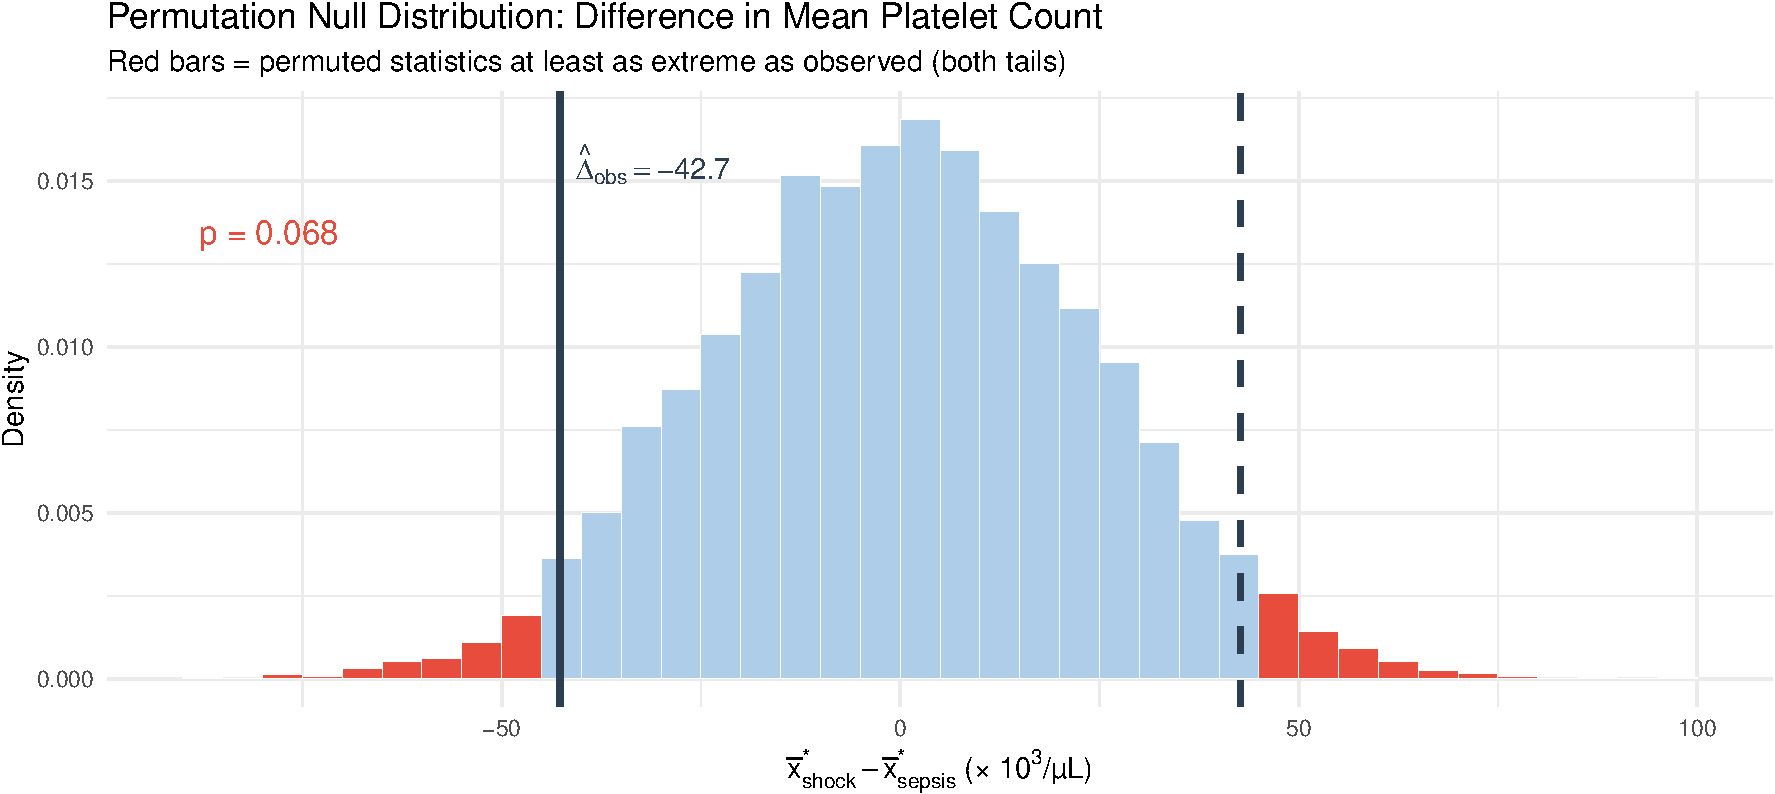
\includegraphics[keepaspectratio]{HW_07_Solutions_files/figure-pdf/unnamed-chunk-25-1.pdf}}




\end{document}
